\documentclass{JFM_Style/jfm}
\usepackage{epstopdf, epsfig}
\usepackage{amsmath}
\usepackage{amssymb}
\usepackage{graphicx}

\newcommand{\ba}{\begin{array}}
\newcommand{\ea}{\end{array}}

\newcommand{\bea}{\begin{eqnarray}}
\newcommand{\eea}{\end{eqnarray}}

\newcommand{\bc}{\begin{center}}
\newcommand{\ec}{\end{center}}

\newcommand{\ds}{\displaystyle}

\newcommand{\bt}{\begin{tabular}}
\newcommand{\et}{\end{tabular}}

\newcommand{\bi}{\begin{itemize}}
\newcommand{\ei}{\end{itemize}}

\newcommand{\bd}{\begin{description}}
\newcommand{\ed}{\end{description}}

\newcommand{\bp}{\begin{pmatrix}}
\newcommand{\ep}{\end{pmatrix}}

\newcommand{\pd}{\partial}
\newcommand{\sech}{\mbox{sech}}

\newcommand{\cf}{{\it cf.}~}

\newcommand{\ltwo}{L_{2}(\mathbb{R}^{2})}
\newcommand{\smooth}{C^{\infty}_{0}(\mathbb{R}^{2})}

\newcommand{\br}{{\bf r}}
\newcommand{\bk}{{\bf k}}
\newcommand{\bv}{{\bf v}}

\newcommand{\gnorm}[1]{\left|\left| #1\right|\right|}
\newcommand{\ipro}[2]{\left<#1,#2 \right>}


\title{Particle Paths in Nonlinear Schr\"{o}dinger Models in the Presence of Linear Shear Currents}
\shortauthor{C.W. Curtis and J.D. Carter and H. Kalisch}

\date{}

\author{C.W. Curtis \aff{1}
  \corresp{\email{ccurtis@mail.sdsu.edu}}, J.D. Carter\aff{2} \and H. Kalisch\aff{3}}

\affiliation{\aff{1}Department of Mathematics and Statistics, San Diego State University, San Diego, CA 92182
\aff{2}Mathematics Department, Seattle University, Seattle, WA 98122
\aff{3}Department of Mathematics, University of Bergen, Bergen, Norway
}

\begin{document}
\maketitle

\begin{abstract}
We investigate the effect of constant vorticity background shear on the properties of wavetrains in deep water.  Using the methodology of \cite{fokas2008}, we derive a higher-order nonlinear Schr\"{o}dinger equation in the presence of shear and surface tension.  We show that the presence of shear induces a strong coupling between the carrier wave and the mean surface displacement.  The effects of the background shear on the modulational instability of plane waves is also studied, where it is shown that shear can suppress instability, though not for all carrier wavelengths in the presence of surface tension.  These results expand upon the findings of \cite{thomas2012nonlinear}.

Using a modification of the Generalized Lagrangian Mean theory in  \cite{andrews} and approximate formulas for the velocity field in the fluid column, explicit, asymptotic approximations for the Lagrangian and Stokes drift velocities are obtained for plane-wave and Jacobi elliptic function solutions of the nonlinear Schr\"odinger equation.  Numerical approximations to particle trajectories for these solutions are found and the Lagrangian and Stokes drift velocities corresponding to these numerical solutions corroborate the theoretical results.

We show that background currents have significant effects on the mean transport properties of waves. In particular, certain combinations of background shear and carrier wave frequency lead to the disappearance of mean surface mass transport.  These results provide a possible explanation for the measurements reported in \cite{smith}.  Our results also provide further evidence of the viability of the modification of the Stokes drift velocity beyond the standard monochromatic approximation, such as recently proposed in \cite{breivik} in order to obtain a closer match to a range of complex ocean wave spectra.
\end{abstract}

\section{Introduction}

Currents are an ubiquitous feature in oceanic dynamics where they are a driving force in the formation and propagation of waves in the ocean.  \cite{helfrich} show that shallow water currents over bathymetric variations are a key mechanism for surface and internal wave generation.  Slowly varying currents likewise act as refractive medium for small-amplitude, linear surface and internal water waves, thereby strongly influencing propagation and dispersion; see \cite{mcwilliams,buhler,young}.  Concominant with this, currents also strongly influence the mean transport properties of waves.  This issue has been extensively studied in \cite{craik1,craik2,craik3,craik4,phillips1,phillips2} where the question of how shear currents excite instabilities and drive mean wave transport in the linear limit has been thoroughly addressed.  However, what is less well understood is the interplay of depth-varying currents with nonlinear surface waves, and how nonlinearity influences the mean transport properties of waves.  

By restricting to the case of a constant-vorticity-shear current, given its relative simplicity, detailed explorations of the existence, shape, stability, and pointwise properties of nonlinear waves in the presence of a current has been studied in a wide number of places such as \cite{freeman,brevik,simmen,pullin2,pullin3,dasilva,baumstein,choi,wahlen,wahlen2,constantin,thomas2012nonlinear,vasan2014pressure} and \cite{nachbin} among many others. In particular, in \cite{thomas2012nonlinear} the impact of vorticity on the modulational instabilities (MIs) of wave trains in deep water was examined.  The MI, which is also known as the Benjamin--Feir instability, is a key factor in the understanding of a number of wave phenomena, and is particularly important in the study of issues such as wave breaking and freak wave formation.  In \cite{thomas2012nonlinear} it is shown that constant vorticity strongly modifies the onset and bandwidth of MIs. Further, it is shown that some currents can even completely suppress MIs, which is a striking result and speaks to the importance of better understanding the role of shear currents in deep water flows.

But there is far less known about how currents impact the transport properties of nonlinear surface waves.  A key measure of the strength of the material transport of surface waves is the Lagrangian drift velocity (LDV), which in the absence of background currents is the mean speed at which fluid parcels travel in a flow, see \cite{longuet}.  An understanding of the LDV, and the associated mean quantity known as the Stokes drift velocity (SDV), is critical in the study of mass and energy transport in oceanic environments, and it has been a central point of investigation in a number of studies such as \cite{mcwilliams,webb,breivik}.  Regarding the impact of constant vorticity currents on the transport properties of surface waves in deep water, the experimental work of \cite{monismith} and the field measurements of \cite{smith} seem to suggest wavetrains on deep water excite Eulerian counter currents which in effect cancel the mean flow induced by the SDV.  These counter currents cancel surface drift in the open ocean such as explained by \cite{smith} and they can even cancel the drift at both the surface and throughout the bulk of fluids in laboratory settings such as found by \cite{monismith}.  To date, there seems to be no theoretical framework explaining the mechanisms behind the development of these currents.  A different but related dilemma emerges in attempts to fit classic, current free, derivations for the SDV in deep water to oceanographic data.  Recently, \cite{breivik} put forward phenomenological modifications to the SDV profile which amount to introducing background currents. They show that the use of these modified SDV profiles is superior to the standard approach of using monochromatic SDV profiles.  However, no physical mechanism is provided which explains the origins of the modifications used in \cite{breivik}.

In order then to better understand the interplay of constant vorticity on deep-water nonlinear-surface flows, we study how a constant vorticity shear profile influences the motion and mean properties of particle paths both at and beneath waves in infinitely deep water.  Our work complements and expands on the shallow and finite depth results found in \cite{wahlen2,constantin,borluk} and \cite{nachbin}.  To do this, we first derive a higher-order nonlinear Schr\"{o}dinger (NLS) model, which we call the Vor-Dysthe (VD) equation, which describes the long temporal and spatial coupling between the nonlinear carrier wave and the mean fluid depth, in effect extending the now classic results of \cite{dysthe} to include constant vorticity and extending the results of \cite{thomas2012nonlinear} to the next asymptotic order.  This is done via the methodology of Ablowitz--Fokas--Musslimani (AFM), see \cite{afm,ashton}, which is a particular case of the more general approach of the Unified Transform Method \cite{fokas2008}.  Using this derivation, we determine not only the appropriate form of the NLS equation, but also the mean-surface height and tangential-surface velocity. We show that the mean-surface height is markedly increased due to the background shear current.  We characterize the impact of constant vorticity and surface tension on MIs, in which we show that surface tension in general prevents there being any vorticity value which completely supresses instability.  This expands on the zero-surface tension results in \cite{thomas2012nonlinear}.  %We note that our derivation method is quite distinct from that in \cite{thomas2012nonlinear} and goes to a higher order.  This provides yet another example of the utility of the AFM formulation.  We then derive dynamical systems which describe the particle paths.

Using these derivations, we provide a description of the impact of constant vorticity shear currents on the LDV and SDV via the techniques of the Generalized Lagrangian Mean (GLM) theory as found in \cite{andrews,buhler}. This approach provides an unambiguous way of computing mean velocities under the influence of depth varying currents, whereby we are then able to explicitly derive formulas for the LDV and SDV for a variety of solutions to the NLS equation. Our method enables the quantification of the combined effect of background shear and wave modulation, and to determine which combinations of background shear and carrier wave frequency produce particularly strong or weak mean flows.  Further, we are able to show which background shear currents quench mean surface flows, thereby providing a potential theoretical explanation for the results presented in \cite{smith}. We also show how one can derive from our model the phenomenological modifications used in \cite{breivik}. 

As stated above, results on the mean transport properties of far more general shear flows have appeared in \cite{craik2, craik3, phillips1, phillips2}, which also explore the existence of transverse instabilities to said shear profiles.  This was done even in the presence of free surfaces; see \cite{phillips1,phillips2}.  However, we note that throughout all of these works, aside from just examing the linear limit of the free surface, thereby disallowing for the study of the slow modulations described by the NLS and VD equations, the computations of mean velocities were done in such a way so that fluctuations around the mean in the horizontal and vertical directions were independent.  While this is certainly appropriate in the bullk of the fluid, as we argue in this paper, this does not make sense at the surface, where one couples the vertical to the horizontal coordinate.  Thus, while we examine a far simpler shear profile, we develop a modification to the standard GLM methodology which treats the free surface in a consistent and more explicit manner.  Likewise, preliminary computations show that our treatement of the surface leads to different mean velocity results than one would get through direct use of the formulas found in say \cite{craik2}, though we note in that paper rigid lids were assumed.  Our predictions of the mean surface velocities are confirmed through the numerical experiments presented in this paper, in particular with regards to the correct dertimination of those constant vorticity values which quench mean transport.  We also note that our formulas for the LDV are in terms of the slow variables underlying the NLS equation, thereby allowing for a clear understanding of the impact of nonlinear wave modulation on the mean transport properties throughout the fluid.  Thus, in this regard, our formulas are nonlinear, though not necessarily of larger amplitude than those found in previous works.  

As a way of confirming our theoretical findings, we discretize the dynamical system describing particle trajectories in the NLS approximation and compute approximations of such trajectories. Our numerical results on the impact of background shear currents on particle paths and the LDV support the results predicted by our theory. We generate the numerical approximations by using using numerical solutions to the VD equation with initial conditions corresponding to the Jacobi elliptic function solutions for both the focusing and defocusing NLS equations to model deep water time-evolving surface wavetrains.  Complementing these results, we also examine using initial conditions corresponding to the defocusing plane-wave solutions of the NLS equation.  Our results show how transport properties are most enhanced for shear currents which at the surface are directed against the carrier wave.  This can occur near what appear to be resonances between nonlinearity and the background shear profile.  Likewise, in the defocusing case we numerically confirm the theoretical predictions made for those balances between vorticity and carrier wave-number which one expects to quench the mean surface drift, thereby providing a possible explanatory mechanism for the results in \cite{smith,breivik,monismith}.  In total, our theoretical and numerical results show that the transport properties of surface waves can be greatly affected by constant vorticity background shear profiles, motivating further study of the impact of rapidly depth-varying currents
on transport properties on nonlinear wavetrains at the free surface.

The outline of the paper is as follows.  The derivations of the VD and NLS equations and the dynamical system describing particle paths is given in Section 2.  The explanations and derivations of the formulas necessary to compute the Stokes drift velocity are given in Section 3.  The numerical results on the particle paths and Stokes drift velocity are in Section 4.
%%%%%%%%%%%%%%%%%%%%%%%%%%%%%%%%%%%%%%%%%%%%%%%%%%%%%%%%%%%%%%%%%%%%%%%%%%%%%%%%%%%
\section{Derivations}
\subsection{Derivation of NLS with Constant Vorticity in Infinite Depth}
We examine the unsteady nonlinear wave propagation over a constant shear current.  To do this, we assume the fluid velocity has the form
\[
{\bf u} = u({\bf x},t)\hat{{\bf x}} + w({\bf x},t)\hat{{\bf z}} = \omega z\hat{{\bf x}} + \nabla \phi,
\]
where $\phi$ is a harmonic function.  We restrict fluid motion to the $(x,z)$-plane, thereby ignoring transverse variations in the $y$ dimension.   Following standard arguments, e.g.~see \cite{ashton}, the dynamics of the fluid can be determined by solving the free boundary value problem
\begin{align}
\Delta \phi = 0, & & -\infty< z < \eta(x,t), \nonumber \\
\eta_{t} +\left(\omega\eta+\phi_{x}\right)\eta_{x} - \phi_{z} = 0, & & z=\eta(x,t), \label{kine}\\
\phi_{t} + \omega\pd_{x}^{-1}\eta_{t} + \frac{1}{2} \left|{\bf
    u}\right|^{2} + g\eta -
\frac{\sigma}{\rho}\pd_{x}\frac{\eta_{x}}{\sqrt{1+\eta_{x}^{2}}}= 0, &
& z=\eta(x,t), \label{bernou}\\
\lim_{z\rightarrow -\infty} \phi_{z} = 0, \nonumber
\end{align}
where $\eta$ represents the free surface displacement, and $g$, $\rho$, and $\sigma$ represent the acceleration due to gravity, the fluid density, and the coefficient of surface tension respectively.

By choosing a characteristic wave height $a$ and wave length $L$, all quantities can be non-dimensionalized via
\begin{align*}
\tilde{x} = \frac{x}{L}, ~\tilde{z} = \frac{z}{L}, ~ \tilde{t} = \sqrt{\frac{g}{L}}~t, ~\omega = \sqrt{\frac{g}{L}}~\tilde{\omega}, \\
\eta = a \tilde{\eta}, ~ \phi  = a\sqrt{gL}~\tilde{\phi} , ~ \epsilon = \frac{a}{L}.
\end{align*}
By following the AFM approach described in \cite{afm,ashton} and dropping the tildes, the kinematic boundary condition, Equation \eqref{kine}, can be written in terms of surface variables alone via the integro-differential equation
\begin{equation}
\int_{\mathbb{R}}dx~e^{-ikx}e^{\epsilon|k|\eta}\left(\eta_{t} +
  \epsilon \omega \eta \eta_{x} + i \mbox{sgn}(k)Q \right) = 0, ~
k\neq 0,
\label{kine2}
\end{equation}
where $Q=q_{x}$, $q(x,t) = \phi(x,\eta(x,t),t)$.  By integrating over $\mathbb{R}$, we are assuming that both $\eta$ and $Q$ decay to zero sufficiently rapidly in the far field.  We can also readily derive a nearly identical expression on domains periodic in the horizontal variable $x$, in which case Equation \eqref{kine2} becomes
\begin{equation}
\int_{-L_{p}/2}^{L_{p}/2}dx~e^{-ikx}e^{\epsilon|k|\eta}\left(\eta_{t} +
  \epsilon \omega \eta \eta_{x} + i \mbox{sgn}(k)Q \right) = 0, ~ k = \frac{2\pi m}{L_{p}}, ~ m\in \mathbb{Z}\backslash{0},
\label{integro1per}
\end{equation}
where $L_p$ is the spatial period.  Throughout the remainder of this section we only present results over the real line $\mathbb{R}$ since identical results can be derived for the periodic case.
Lastly, we note that if in Equation \eqref{kine2} we approach $k=0$ from both the left and the right, we get the equations
\[
\int_{\mathbb{R}}dx \left(\eta_{t} + i Q \right) = 0, ~ \int_{\mathbb{R}}dx \left(\eta_{t} - i Q \right) = 0.
\]
Thus we get the identities
\begin{align}
\p_{t}\int_{\mathbb{R}} dx ~\eta(x,t) & = 0, \label{zavsurf}\\
\int_{\mathbb{R}} dx ~Q(x,t) & = 0. \label{zavpot}
\end{align}

Taylor expanding Equation (\ref{kine2}) up to $\mathcal{O}(\epsilon^3)$ for $k\neq 0$ gives
\begin{multline}
\int_{\mathbb{R}}dx~e^{-ikx}\left(1 + \epsilon |k|\eta + \frac{\epsilon^{2}|k|^{2}\eta^{2}}{2} + \frac{\epsilon^{3}|k|^{3}\eta^{3}}{6}\right)\left(\eta_{t} + i \mbox{sgn}(k)Q \right) \\
+ \epsilon \omega \int_{\mathbb{R}}dx~e^{-ikx}\left(1 + \epsilon |k|\eta + \frac{\epsilon^{2}|k|^{2}\eta^{2}}{2}\right) \eta \eta_{x} = 0.
\label{integro1}
\end{multline}
Transforming into surface variables and Taylor expanding Equation \eqref{bernou}, Bernoulli's equation, up to $\mathcal{O}(\epsilon^3)$ gives
\begin{multline}
Q_{t} + \omega \eta_{t} + \eta_{x} - \tilde{\sigma}\eta_{xxx} + \frac{\epsilon}{2}\pd_{x}\left(-\eta_{t}^{2} + (Q+\omega \eta)^{2} \right)\\
+ \epsilon^{2}\pd_{x}\left( \frac{3}{2}\tilde{\sigma}\eta_{x}^{2}\eta_{xx} - \eta_{t}\eta_{x} \left(Q  + \omega \eta \right) \right) - \frac{\epsilon^{3}}{2}\eta_{x}^{2}\left((\omega\eta+Q)^{2}-\eta_{t}^{2}\right) = 0,
\label{berexp}
\end{multline}
where the reciprocal of the Bond number, $\tilde{\sigma}$, is given by
\[
\tilde{\sigma} = \frac{\sigma}{\rho g L^2}.
\]
We note that we have tacitly assumed $\omega = \mathcal{O}(1)$.  In physical terms, this implies that $\omega$ is comparable to the natural time scale of this problem, $\sqrt{L/g}$.  If we were to assume $\omega$ were of larger magnitude, the problem would no longer be weakly nonlinear and thus would be much less amenable to asymptotic analysis.  Therefore, throughout the remainder of the paper, we assume that the vorticity is not too large.

The nonlocality in the full equations comes from the Hilbert transform, $\mathcal{H}$, defined by
\[
\mathcal{H}f = \frac{1}{2\pi}\int_{\mathbb{R}}dk~ e^{ikx}  i\mbox{sgn}(k) \hat{f}(k),
\]
where $\hat{f}(k)$ is the Fourier transform of $f(x)$ defined by
\[
\hat{f}(k) = \int_{\mathbb{R}}dx~ e^{-ikx}f(x).
\]
In other words, $\mathcal{H}$ is the operator with symbol $i\mbox{sgn}(k)$.  Given that
\[
\mbox{sgn}(k_{0} + \epsilon k) = \mbox{sgn}(k_{0})\mbox{sgn}\left( 1 + \frac{\epsilon k}{k_{0}}\right),
\]
assuming $\hat{f}(k)$ is a function of rapid decay, see \cite{folland},  and assuming $k_{0}\gg \epsilon$ gives
\begin{align}
\mathcal{H}\left( f(\epsilon x) e^{ik_{0}x} \right)& =
\frac{e^{ik_{0}x}}{2\pi}\int_{\mathbb{R}}dk~ e^{ik\epsilon x}
i\mbox{sgn}(k_{0}+\epsilon k) \hat{f}(k)\nonumber \\ & \sim i\mbox{sgn}(k_{0})e^{ik_{0}x}f(\epsilon x).\nonumber
\end{align}
with the difference being exponentially small.  On the other hand, if $k_{0}=0$, then
\[
\mathcal{H}\left( f(\epsilon x) \right) = \frac{1}{2\pi}\int_{\mathbb{R}}dk~ e^{ik\epsilon x}  i\mbox{sgn}(k) \hat{f}(k) = (\mathcal{H}f)(\epsilon x).
\]
Thus, the Hilbert transform does not have any significant effect on the multiple scales ans\"{a}tze made below.

Equation (\ref{integro1}) readily leads to a recursive formula for the surface velocity potential $Q$ of the form
\begin{equation}
Q = \mathcal{H}\p_{t}\eta + \epsilon R_{1} + \epsilon^{2} R_{2} + \epsilon^{3} R_{3},
\label{Qexp}
\end{equation}
where
\begin{align*}
R_{1}= & \mathcal{H}\p_{x}\left(\eta\mathcal{H}\p_{t}\eta+ \frac{\omega}{2}\eta^{2} - \frac{1}{2}\mathcal{H}\p_{t}\eta^{2} \right),\\
R_{2}= & \mathcal{H}\p_{x}\left(\eta R_{1} \right) - \mathcal{H}\p_{x}^{2}\left(\frac{1}{6}\p_{t}\eta^{3} + \frac{\omega}{3}\mathcal{H}\eta^{3} + \frac{1}{2}\mathcal{H}(\eta^{2}\mathcal{H}\p_{t}\eta)\right),\\
R_{3} = & \mathcal{H}\p_{x}\left(\eta R_{2} \right) + \frac{1}{2}\p_{x}^{2}\left(\eta^{2}R_{1}\right) + \mathcal{H}\p_{x}^{3}\left(\frac{1}{24}\mathcal{H}\p_{t}\eta^{4} - \frac{1}{6}\eta^{3}\mathcal{H}\p_{t}\eta - \frac{\omega}{8}\eta^{4}\right).
\end{align*}
Coupling this to Equation \eqref{berexp} gives a single scalar equation defined entirely in terms of the surface height $\eta$.  Now, use the ansatz
\begin{multline}
\eta(x,t) = \epsilon \eta_{0}(\xi,\tau) + \eta_{1}(\xi,\tau)e^{i\theta} +  \eta_{1}^{\ast}(\xi,\tau)e^{-i\theta} + \epsilon\left(\eta_{2}(\xi,\tau)e^{2i\theta} +  \eta_{2}^{\ast}(\xi,\tau)e^{-2i\theta}\right) \\
+ \epsilon^{2}\left(\eta_{3}(\xi,\tau)e^{3i\theta} +  \eta_{3}^{\ast}(\xi,\tau)e^{-3i\theta}\right)  + \epsilon^{3}\left(\eta_{4}(\xi,\tau)e^{4i\theta} +  \eta_{4}^{\ast}(\xi,\tau)e^{-4i\theta}\right) + \cdots
\label{nlssurfexp}
\end{multline}
where
\begin{equation}
\theta = k_{0}x + \Omega t, ~ \xi = \epsilon(x + c_{g}t), ~ \tau = \epsilon^{2}t.
\label{xidef}
\end{equation}
We note that using integration by parts shows that terms of the form $\eta_{m}e^{im\theta}$ satisfy 
\[
\int_{\mathbb{R}} dx ~ \eta_{m}(\xi,\tau) e^{im\theta}  = \mathcal{O}(\epsilon^{j}), ~ j\geq 1,~ m>0,
\]
which is to say that these terms are vanishingly small in an asymptotic sense.  Thus, asymptotically, Equation \eqref{zavsurf} becomes
\begin{equation}
\p_{\tau}\int_{\mathbb{R}} d\xi ~ \eta_{0}(\xi,\tau) = 0.
\label{zavzmean}
\end{equation}

By expanding and matching terms in the fundamental harmonic, $e^{i\theta}$, at $\mathcal{O}(1)$ we obtain the linear dispersion relation,
\begin{equation}
\Omega_{\pm}(k_{0},\omega)  = \frac{1}{2}\left(s\omega \pm \sqrt{\omega^{2} + 4|k_{0}|(1+\tilde{\sigma}k_{0}^{2})}\right),
\label{LDR}
\end{equation}
and at $\mathcal{O}(\epsilon)$ we find that
\[
c_{g} = \frac{1+3\tilde{\sigma}k_{0}^{2}}{2s\Omega - \omega},
\]
where $s=\mbox{sgn}(k_{0})$.  We note that Equation (\ref{LDR}) establishes that $\Omega_{+}(k_{0},\omega) > 0$ and $\Omega_{-}(k_{0},\omega) < 0$ for $k_{0}\neq0$.  Throughout the remainder of the paper, $\Omega$ always denotes the positive branch, $\Omega_{+}$.  By looking at the second harmonic, $e^{2i\theta}$, we find that
\[
\eta_{2} = \ell_{0}\eta_{1}^{2} + i\epsilon\ell_{1}\eta_{1}\p_{\xi}\eta_{1}+\mathcal{O}(\epsilon^2),
\]
where
\begin{align*}
\ell_{0} = & -\frac{k_{0}\left(\omega^{2}+2\Omega^{2}-4s\omega\Omega\right)}{2(k_{0} + \omega\Omega - 2s\Omega^{2} + 4\tilde{\sigma}k_{0}^{3})},\\
\ell_{1} = & \frac{\left(2c_{g}k_{0}(\Omega-s\omega)-2s\omega\Omega + \Omega^{2} + \omega^{2}/2\right)+(1+\omega c_{g} + 12k_{0}^{2}\tilde{\sigma}-4sc_{g} \Omega)\ell_{0}}{k_{0} + \omega\Omega - 2s\Omega^{2} + 4\tilde{\sigma}k_{0}^{3}}.
\end{align*}
By then going up to $\mathcal{O}(\epsilon^{3})$, we get the following coupled system describing the slow spatial and temporal modulation due to the interaction of the leading harmonic term $\eta_{1}$ and the mean surface height $\eta_{0}$
\begin{multline}
\epsilon c_{g}^{2}\mathcal{H}\p_{\xi}^{2}n_{0} + (1+\omega c_{g})\p_{\xi}\eta_{0} + \epsilon \omega \p_{\tau} n_{0} + \omega\left(\omega-2s\Omega\right)\p_{\xi}\left|\eta_{1}\right|^{2}\\
+\epsilon\left(c_{g}(\omega-2s\Omega)\mathcal{H}\p_{\xi}^{2}\left|\eta_{1}\right|^{2} + is\omega c_{g}\left(\eta_{1}^{\ast}\p_{\xi}^{2}\eta_{1}-\eta_{1}\p_{\xi}^{2}\eta_{1}^{\ast}\right) \right) = 0,
\label{zaveq}
\end{multline}

\begin{multline}
(\omega-2s\Omega)\p_{\tau}\eta_{1} + i(c_{g}^{2}s-3k_{0}\tilde{\sigma})\p_{\xi}^{2}\eta_{1} + 2i\epsilon s c_{g}\p^{2}_{\xi\tau}\eta_{1} - \epsilon\tilde{\sigma} \p^{3}_{\xi}\eta_{1} \\
+ ik_{0}\omega\left(\omega-2s\Omega\right)\eta_{0}\eta_{1} +
i \alpha_{0}\left|\eta_{1}\right|^{2}\eta_{1}
+ \epsilon\alpha_{1}\left|\eta_{1}\right|^{2}\p_{\xi}\eta_{1}
+ \epsilon\alpha_{2}\eta_{1}^{2}\p_{\xi}\eta^{\ast}_{1} + \\
\epsilon i\alpha_{3}\eta_{1}\mathcal{H}\p_{\xi}\left|\eta_{1}\right|^{2}
 + \epsilon \omega(\omega-2s\Omega-|k_{0}|c_{g})\eta_{1}\p_{\xi}\eta_{0} + \epsilon\omega(\omega-2s\Omega-2|k_{0}|c_{g})\eta_{0}\p_{\xi}\eta_{1} \\
+ \epsilon ik_{0}c_{g}(\omega-2s\Omega)\eta_{1}\mathcal{H}\p_{\xi}\eta_{0} = 0,
\label{mnls}
\end{multline}
where
\begin{align*}
\alpha_{0} = & k_{0}^{2}\left(-\frac{3}{2}k_{0}^{3}\tilde{\sigma} + 2s\Omega^{2}-s\omega^{2}\right) + \ell_{0}k_{0}\left(\omega^{2}+2\Omega^{2}-4s\omega\Omega\right),\\
\alpha_{1} = & k_{0}\left(4c_{g}|k_{0}|\Omega - 9\tilde{\sigma}k_{0}^{3}+6s\Omega^{2}-3s\omega^{2}\right) \\
& + \ell_{0} \left(2\omega^{2}+4\Omega^{2}-8s\omega\Omega+4k_{0}c_{g}(\Omega-s\omega)\right) + \ell_{1}k_{0}\left(4s\omega\Omega-2\Omega^{2}-\omega^{2}\right),\\
\alpha_{2} = & k_{0}\left(-\frac{3}{2}k_{0}^{3}\tilde{\sigma}+2s\Omega^{2}-s\omega^{2}\right)  + \ell_{0}\left(\omega^{2} + 2\Omega^{2}-4s\omega\Omega\right),\\
\alpha_{3} = & k_{0}\left(\omega-2s\Omega\right)^{2}.
\end{align*}

By solving Equation \eqref{zaveq} to leading order and using Equation \eqref{zavzmean}, we find that
\begin{equation}
\eta_{0}(\xi,\tau) = \frac{\omega(2s\Omega-\omega)}{1+\omega c_{g}}\left|\eta_{1}\right|^{2}(\xi,\tau) +\mathcal{O}(\epsilon),
\label{zavsol}
\end{equation}
Likewise, from \eqref{mnls} at this order, and using the leading order solution for the mean height, $\eta_{0}$, gives the time-dependent NLS equation
\begin{equation}
i\p_{\tau}\eta_{1} + \alpha_{nl}\left|\eta_{1}\right|^{2}\eta_{1} + \alpha_{d}\p_{\xi}^{2}\eta_{1} = 0,
\label{NLSS}
\end{equation}
where
\begin{align*}
\alpha_{d}(k_{0},\omega) = & \frac{(c^2_{g} - 3|k_{0}|\tilde{\sigma})}{2\Omega-s\omega},\\
\alpha_{nl}(k_{0},\omega) = & \frac{k_{0}\left( sk_{0}^{3}\left(8 + \tilde{\sigma}k_{0}^{2} + 2(\tilde{\sigma}k_{0}^{2})^{2}\right) + \omega \alpha_{v}\right)}{\left(2s\Omega -\omega\right)(1+c_{g}\omega)\left(4\Omega^2-s(2k_{0}(1+4\tilde{\sigma}k_{0}^{2})+2\omega\Omega)\right)},
\end{align*}
and
\begin{align*}
\alpha_{v}(k_{0},\omega)= & s(c_g k_0  - 2\Omega ) \omega^4 + k_{0}(4 k_{0}^{2} s \tilde{\sigma} + 2 \Omega c_g  -s) \omega^3 \\
& + k_{0}(16 c_g k_{0}^{3} \tilde{\sigma} - 8 \Omega k_{0}^{2} \tilde{\sigma} + 10 c_g k_{0} - 6 \Omega) \omega^2 \\
& -  k_{0}^{2}(15 \Omega c_g k_0^2 s \tilde{\sigma} - 16 k_{0}^{4} \tilde{\sigma}^2 - 24 k_{0}^{2} \tilde{\sigma} - 2 ) \omega \\
& + k_{0}^{3}(2 c_g k_{0}^{4} s \tilde{\sigma}^2 + c_g k_{0}^{2} s \tilde{\sigma} - 15 \Omega k_{0}  s \tilde{\sigma} + 8c_g s).
\end{align*}
Note, our results for the NLS equation agree with those in \cite{afm} for $\omega=0$, and they agree with the results in \cite{thomas2012nonlinear} for $\tilde{\sigma}=0$.  Further, all of our results in this section are derived with the aid of the computer algebra system SAGE.

We readily see that we can go to higher order in the mean term using Equation \eqref{zaveq} and the expansion
\[
\eta_{0}(\xi,\tau) = \frac{\omega(2s\Omega-\omega)}{1+\omega c_{g}}\left|\eta_{1}\right|^{2}(\xi,\tau) + \epsilon \eta_{01}(\xi,\tau) + \mathcal{O}(\epsilon^{2}),
\]
which gives
\[
\eta_{01}= \frac{c_{g}(2s\Omega-\omega)}{(1+\omega c_{g})^{2}}\mathcal{H}\p_{\xi}\left|\eta_{1}\right|^{2} + \frac{i\omega}{1+\omega c_{g}}\left(\frac{\alpha_{d}\omega(2s\Omega-\omega)}{1+\omega c_{g}} + s c_{g} \right) \left(\eta_{1}\p_{\xi}\eta_{1}^{\ast} - \eta_{1}^{\ast}\p_{\xi}\eta_{1} \right) 
\]
Thus, we can finally write Equation \eqref{mnls} in terms of $\eta_{1}$ alone so that we get 
\begin{multline}
(\omega-2s\Omega)\p_{\tau}\eta_{1} + i(c_{g}^{2}s-3k_{0}\tilde{\sigma})\p_{\xi}^{2}\eta_{1} + 2i\epsilon s c_{g}\p^{2}_{\xi\tau}\eta_{1} - \epsilon\tilde{\sigma} \p^{3}_{\xi}\eta_{1} \\
- i \alpha_{nl}(\omega-2s\Omega)\left|\eta_{1}\right|^{2}\eta_{1}
+ \epsilon \tilde{\alpha}_{1}\left|\eta_{1}\right|^{2}\p_{\xi}\eta_{1}
+ \epsilon\tilde{\alpha}_{2}\eta_{1}^{2}\p_{\xi}\eta^{\ast}_{1} + 
\epsilon i\tilde{\alpha}_{3}\eta_{1}\mathcal{H}\p_{\xi}\left|\eta_{1}\right|^{2}= 0.
\label{dysthe}
\end{multline}
Obtaining the coefficients $\tilde{\alpha}_{j}$ is straightforward, and thus we omit writing them down for the sake of brevity.  We call Equation \eqref{dysthe} the Vor-Dysthe (VD) equation.  By solving it, we in effect find the next order correction to the NLS equation, and thus, by combining with our previous results, we can find $\eta$ up to $\mathcal{O}(\epsilon^{2})$ on a $\mathcal{O}(1/\epsilon^{2})$ timescale.  This becomes a critical feature necessary to ensure the accuracy of our numerics in Section 4.  

For the NLS equation, the case in which $\alpha_{d}$ and $\alpha_{nl}$ have the same sign is known as the `focusing' case while the case in which they have opposite signs is known as the `defocusing' case.  These two cases are qualitatively different.  In the focusing case, the trivial-phase Jacobi elliptic solutions are given by
\begin{equation}
\eta_{1}(\xi,\tau) = \kappa\beta \sqrt{\frac{2\alpha_{d}}{\alpha_{nl}}}~\mbox{cn}(\beta \xi;\kappa)e^{-i\alpha_{d}\beta^{2}(1-2\kappa^2)\tau},
\label{cnsolns}
\end{equation}
where $0\le\kappa\le1$ is the elliptic modulus and $\beta$ is a positive lengthscale parameter.  In the $\kappa \rightarrow 1$ limit, these solutions limit to the `bright' soliton solutions
\[
\eta_{1}(\xi,\tau)=\beta \sqrt{\frac{2\alpha_{d}}{\alpha_{nl}}}~\mbox{sech}(\beta \xi)e^{i\alpha_{d}\beta^{2}\tau}.
\]
In the defocusing case, the trivial-phase Jacobi elliptic solutions are given by
\begin{equation}
\eta_{1}(\xi,\tau) = \kappa\beta \sqrt{-\frac{2\alpha_{d}}{\alpha_{nl}}}~\mbox{sn}(\beta \xi;\kappa) e^{-i\alpha_{d}\beta^{2}(1+\kappa^2)\tau}.
\label{snsolns}
\end{equation}
In the $\kappa\rightarrow1$ limit, these solutions limit to the `dark'
soliton solutions
\[
\eta_{1}(\xi,\tau)=\beta \sqrt{-\frac{2\alpha_{d}}{\alpha_{nl}}}~ \mbox{tanh}(\beta \xi)  e^{-2i\alpha_{d}\beta^{2}\tau}.
\]
The elevated profile of the magnitude of the bright soliton is qualitatively different from the depressed profile of the magnitude of the dark soliton.  This distinction typifies the difference between the behavior of the focusing and defocusing cases.  Note that in order for $\eta(x,t)$ to be periodic when Jacobi elliptic functions are used, the following restriction must be enforced
\begin{equation}
k_{0} = \frac{\pi \epsilon m}{2K(\kappa)},~ m\in \mathbb{Z},
\label{jacwavnum}
\end{equation}
where $K(\kappa)$ is the complete elliptic integral of the first kind.
%%%%%%%%%%%%%%%%%%%%%%%%%%%%%%%%%%%%%%%%%%%%%%%%%%%%%%%%%%%%%%%%%%%%%%%%%%%%%%%%%%%
\subsection{Modulational Instabilities and Currents in Infinite Depth}
The plane-wave, or Stokes wave, solutions of the NLS equation are given by
\begin{equation}
\eta_{1}(\xi,\tau) = A e^{i\alpha_{nl}A^{2}\tau},
\end{equation}
where $A>0$ is a real constant.  Complementing the results in \cite{thomas2012nonlinear}, we study the stability of these solutions by considering perturbed solutions of the form
\begin{equation}
\eta_{1p}(\xi,\tau) = \Big{(}A +\mu \big{(}u_{p}(\xi,\tau)+iv_{p}(\xi,\tau)\big{)} +\mathcal{O}(\mu^2)\Big{)}\mbox{e}^{i\alpha_{nl}A^{2}\tau},
\label{pert}
\end{equation}
where $\mu$ is a small real parameter and $u_{p}$ and $v_{p}$ are real-valued functions.  Substituting (\ref{pert}) into the NLS equation and linearizing gives
\[
\pd_{\tau}\bp u_{p}\\ v_{p}\ep = \bp 0 & -\alpha_{d}\pd_{\xi}^{2} \\ \alpha_{d}\pd_{\xi}^{2} + 2A^{2}\alpha_{nl} & 0 \ep \bp u_{p} \\ v_{p} \ep.
\]
Separating variables, applying a Fourier transform in $\xi$, and introducing the $\xi$ wave number $l$, establishes that NLS plane-wave solutions are unstable with respect to the modulational instabilities (MIs) if
\[
0 < l^{2} \leq 2\frac{\alpha_{nl}}{\alpha_{d}}A^{2}.
\]
This reduces to the classic requirement that MIs are suppressed if the coefficients of dispersion and nonlinearity have opposite signs (i.e.~the defocusing case).

Figure \ref{fig:miplot} shows the values of $\omega$ and $k_{0}$ for which MIs exist (white areas) or not (black areas) for $\tilde{\sigma}=10^{-3}$ in Figure \ref{fig:miplot} (a), $\tilde{\sigma}=10^{-5}$ in Figure \ref{fig:miplot} (b), $\tilde{\sigma}=10^{-5}$ in Figure \ref{fig:miplot} (c), and $\tilde{\sigma}=0$ in Figure \ref{fig:miplot} (d).   Note, the scale of the axes changes from Figures \ref{fig:miplot} (a) and (b) to (c) and (d).  Further, while we assumed that $\omega = \mathcal{O}(1)$ in our derivation of the NLS equation, to see the impact of surface tension and its connection to MI, we have had to plot on an exaggerated scale in Figure \ref{fig:miplot}.  As can be seen, in the presence of surface tension, there does not appear to be a value of $\omega$ that suppresses MIs across all wave numbers.  This is in contrast to the zero surface tension case, in which if $k_{0}\omega>0$ and the magnitude of the shear is sufficiently large, then the MI is suppressed across all wave numbers.  As can be seen by comparing Figures \ref{fig:miplot} (a), (b), and (c), larger surface tension facilitates the transitions between regions in which the MI is or is not suppressed for relatively smaller values of carrier wavenumber and shear magnitude.  This expands on the results in \cite{thomas2012nonlinear}, which did not consider the effect of surface tension.  Throughout the rest of the paper we take $\tilde{\sigma}=10^{-5}$ which corresponds to supposing a characteristic wave length $L\sim 1m$.
\begin{figure}
\centering
\begin{tabular}{cc}
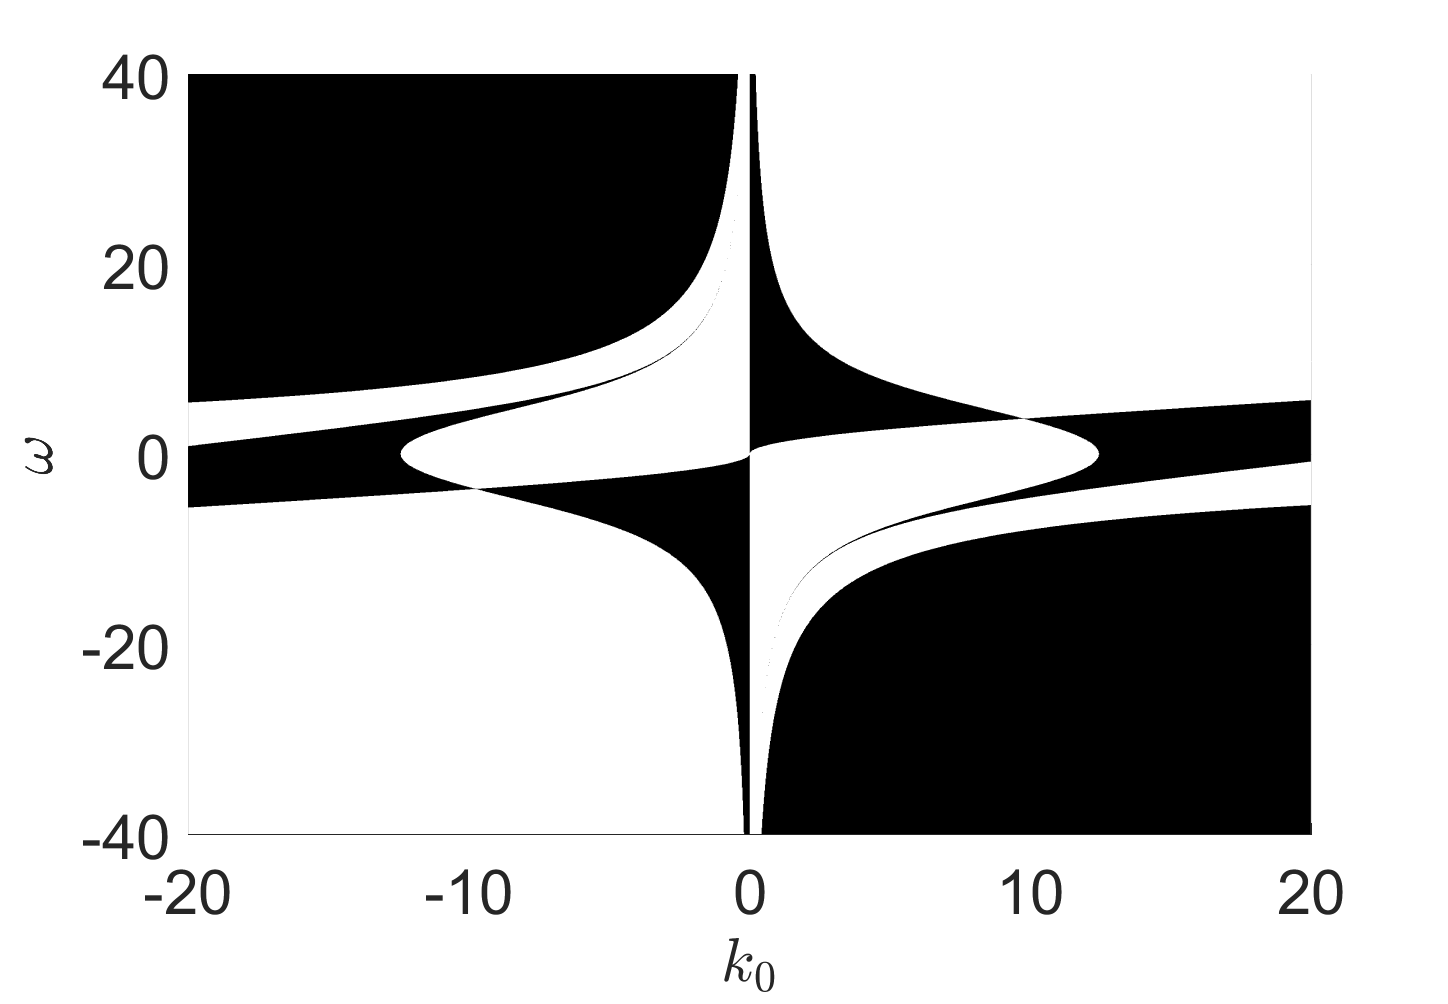
\includegraphics[width=.48\textwidth]{foc_defoc_pos_cut} & 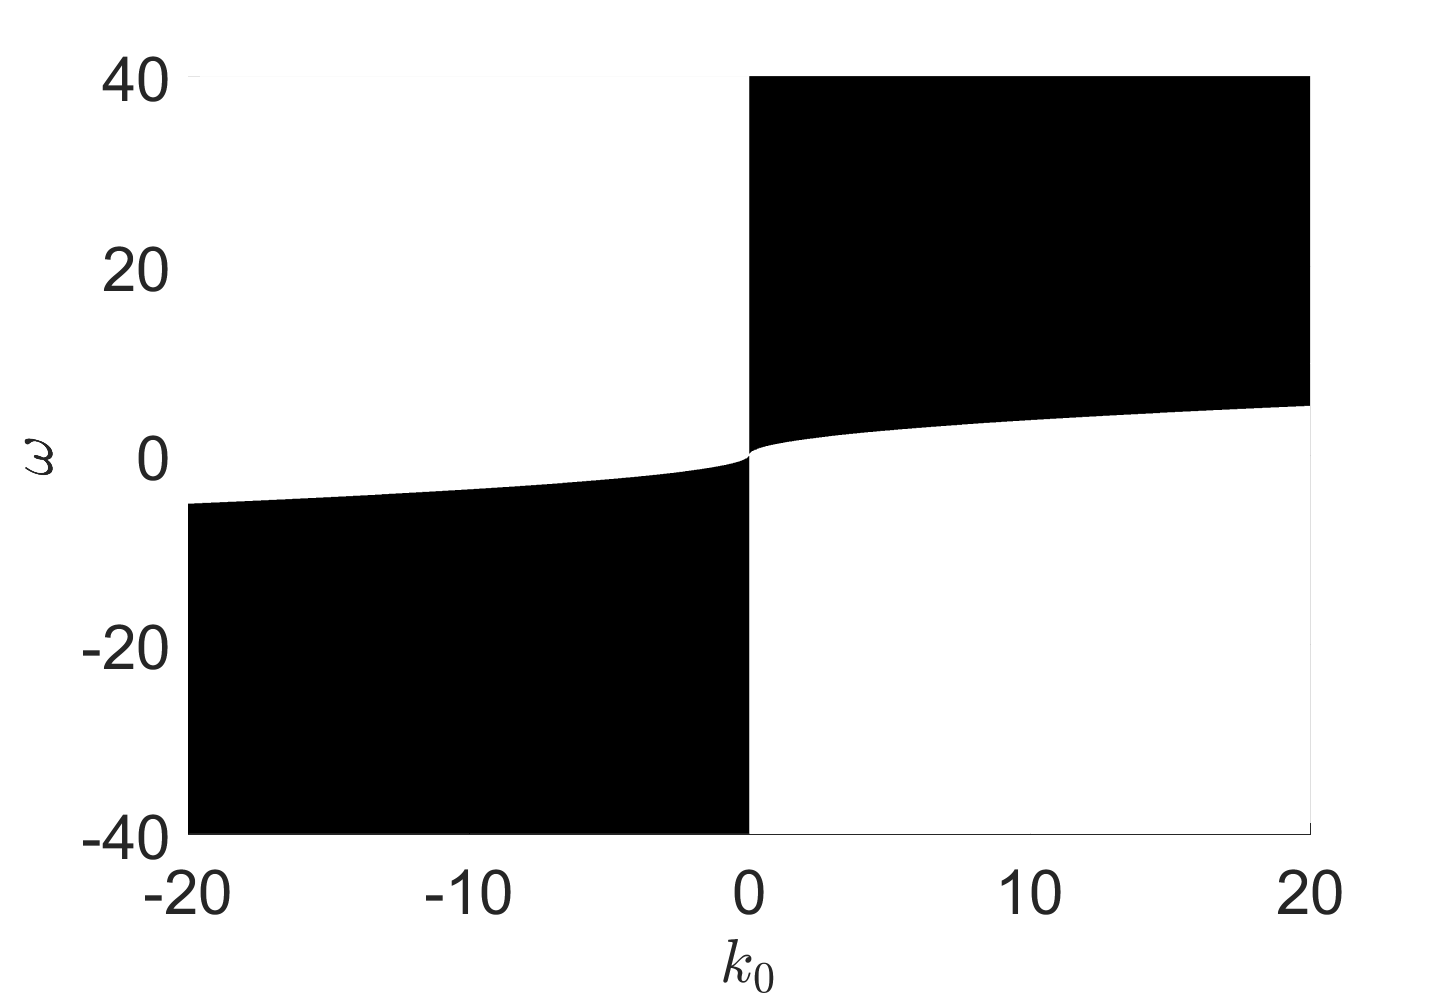
\includegraphics[width=.48\textwidth]{foc_defoc_pos_cut_sig_1en5}\\
(a) & (b)\\
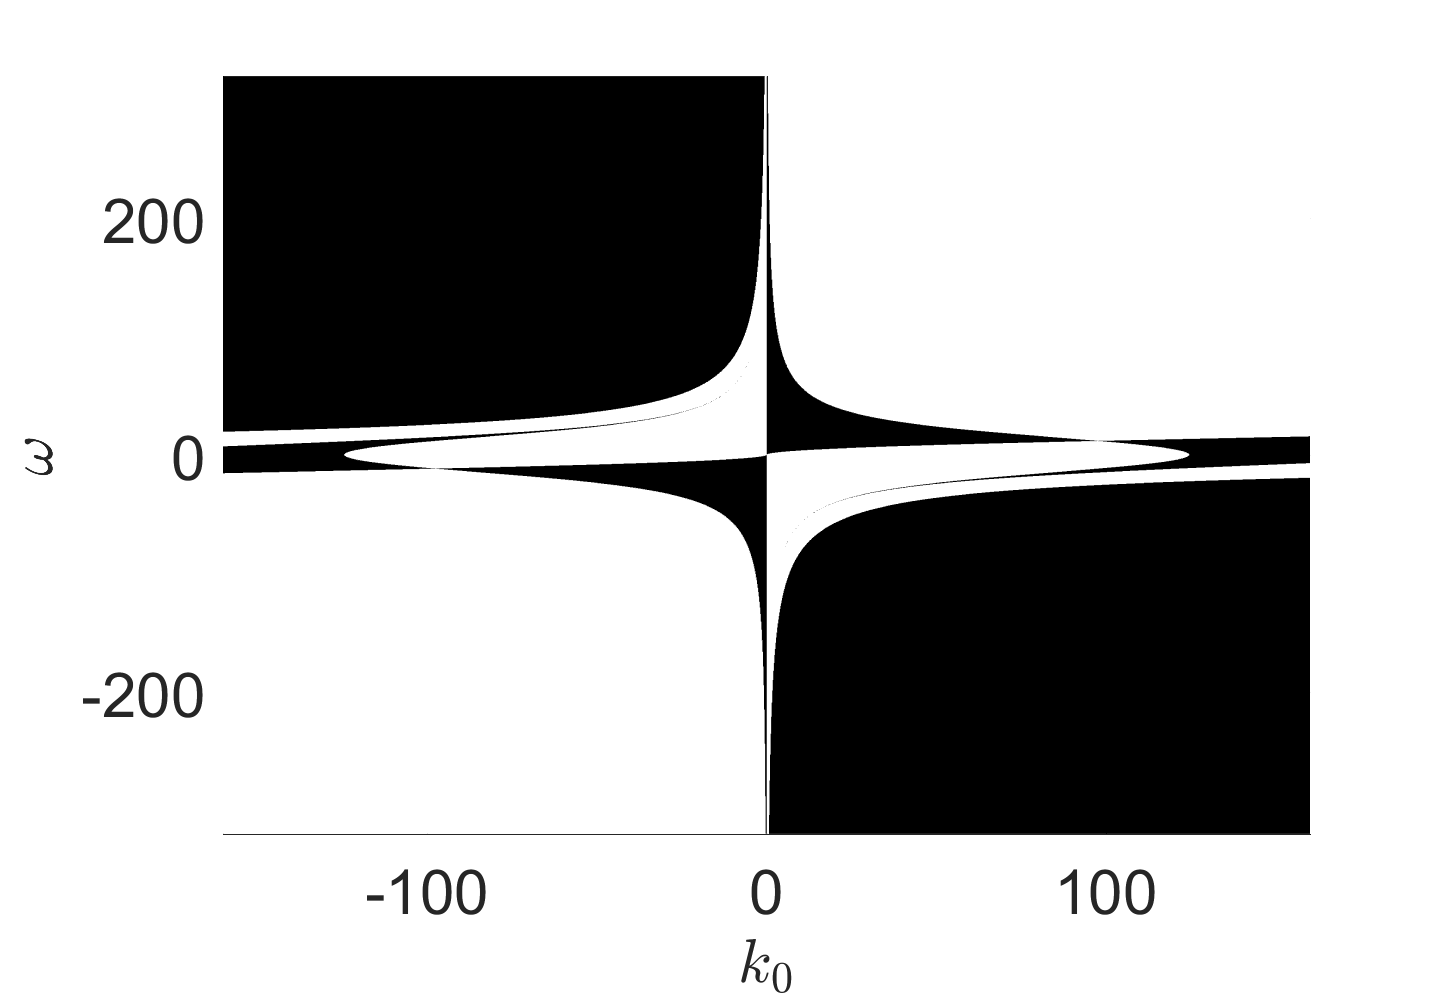
\includegraphics[width=.48\textwidth]{foc_defoc_pos_cut_sig_1en5_wide} & 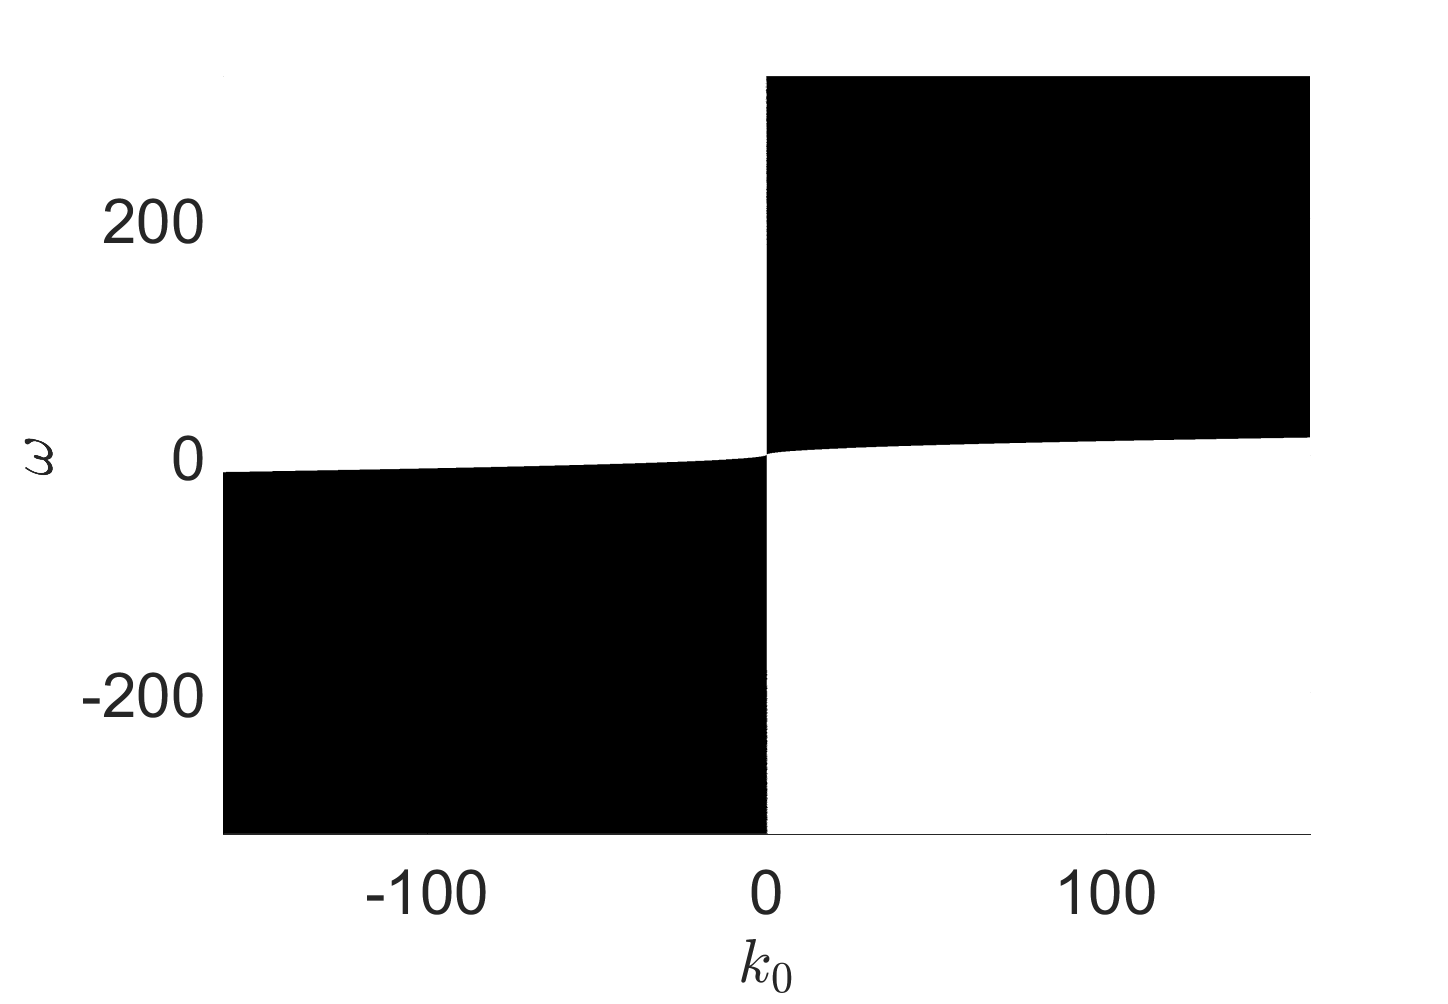
\includegraphics[width=.48\textwidth]{foc_defoc_pos_cut_sig_0_wide}\\
(c) & (d)
\end{tabular}
\caption{\small {\it MIs exist} - white, \small{\it MIs suppressed} - black, for $\tilde{\sigma}=10^{-3}$ (a), $\tilde{\sigma}=10^{-5}$ (b), $\tilde{\sigma}=10^{-5}$ (c), and $\tilde{\sigma}=0$ (d).  Note the change in scale of the axes in (c) and (d) relative to (a) and (b).}
\label{fig:miplot}
\end{figure}

Per our convention of taking the fast phase, $\theta(x,t)$, to be
\[
\theta(x,t) = k_{0}x + \Omega(k_{0},\omega) t,
\]
if $k_{0}\Omega(k_{0},\omega)>0$, then the carrier wave propagates to the left, and if $k_0 \Omega(k_{0},\omega)<0$, then the carrier wave propagates to the right.  Figures \ref{fig:miplot}(a) and (c) then show that MIs are generally suppressed when the shear current at the surface is co-propagating with respect to the carrier wave with sufficient strength which is inversely related to the carrier wavenumber.  Thus, in order to suppress most MIs, we need either relatively high carrier wave numbers for relatively weak shear currents, or relatively strong shear currents for relatively low carrier wave numbers.  The regions in Figures \ref{fig:miplot}(a) and (c) in which counter-propagating sheer currents suppress MIs are more complicated in nature, though one can argue that counter-propagating currents generally exacerbate MIs, especially with increasing shear strength.   
%%%%%%%%%%%%%%%%%%%%%%%%%%%%%%%%%%%%%%%%%%%%%%%%%%%%%%%%%%%%%%%%%%%%%%%%%%%%%%%%%%%
\subsection{Derivation of Velocity Formulas}
In non-dimensional coordinates, the position of a given fluid particle, $(x(t),z(t))$, is defined by the dynamical system
\begin{align}
\begin{split}
\dot{x} = \omega z + \epsilon \phi_{x}(x,z,t), ~~~~ \dot{z} = \epsilon\phi_{z}(x,z,t),\\
x(0) =x_0,~~~~ z(0)=z_0.
\end{split}
\label{system}
\end{align}
Therefore, in order to track the motion of a fluid particle, both $\phi_x$ and $\phi_z$ must be known throughout the fluid domain.  In order to determine asymptotic formulas for these quantities, let
\begin{equation}
\phi_{x}(x,z,t) = \frac{1}{2\pi}\int_{\mathbb{R}}dk~ e^{ikx} A(k,t)e^{|k|z},
\label{phix}
\end{equation}
\begin{equation}
\phi_{z}(x,z,t) = \frac{1}{2\pi}\int_{\mathbb{R}}dk~ e^{ikx} B(k,t)e^{|k|z}.
\label{phiz}
\end{equation}
Expanding $e^{\epsilon \eta |k|}$ in Equations (\ref{phix}) and (\ref{phiz}) gives
\begin{align}
\left.\phi_{x}\right|_{z=\epsilon\eta} = & \tilde{A}(x,t) - \epsilon\eta\mathcal{H}\pd_{x}\tilde{A} +\mathcal{O}(\epsilon^{2}),\label{phixsurfsol}\\
\left.\phi_{z}\right|_{z=\epsilon\eta} = & \tilde{B}(x,t) - \epsilon\eta\mathcal{H}\pd_{x}\tilde{B} +\mathcal{O}(\epsilon^{2}),\label{phizsurfsol}
\end{align}
where
\[
\tilde{A}(x,t) = \frac{1}{2\pi}\int_{\mathbb{R}}dk~ e^{ikx} A(k,t), ~~~~ \tilde{B}(x,t) = \frac{1}{2\pi}\int_{\mathbb{R}}dk~ e^{ikx} B(k,t).
\]

The surface boundary conditions give
\begin{align*}
\left.\phi_{x}\right|_{z=\epsilon\eta} = & \frac{Q-\epsilon\eta_{x}(\eta_{t}+\epsilon\omega\eta\eta_{x})}{1+\epsilon^{2}\eta_{x}^{2}},\\
\left.\phi_{z}\right|_{z=\epsilon\eta} = & \frac{\eta_{t}+\epsilon \left(Q+\omega\eta\right)\eta_{x}}{1+\epsilon^{2}\eta_{x}^{2}}.
\end{align*}
Substituting the expansions in Equations \eqref{Qexp} and \eqref{nlssurfexp} into these equations and using the results obtained during the derivation of the NLS equation gives
\begin{align}
\left.\phi_{x}\right|_{z=\epsilon\eta} = & -2\epsilon k_{0}\Omega \left|\eta_{1} \right|^{2} + \left(-s\Omega\eta_{1} + i\epsilon s c_{g}\pd_{\xi}\eta_{1} \right)e^{i\theta} \nonumber \\
& - \epsilon(2s\Omega\eta_{2}+ k_{0}(s\omega-\Omega) \eta_{1}^{2})e^{2i\theta} + \mbox{c.c.} + \mathcal{O}(\epsilon^{2}),\label{phisurfsollhsx}\\
\left.\phi_{z}\right|_{z=\epsilon\eta} = & (i\Omega \eta_{1}+\epsilon c_{g}\pd_{\xi}\eta_{1})e^{i\theta} + i\epsilon(2\Omega\eta_{2} + k_{0}(\omega-s\Omega)\eta_{1}^{2})e^{2i\theta} + \mbox{c.c.} + \mathcal{O}(\epsilon^{2}). \label{phisurfsollhsz}
\end{align}
This motivates the expansions
\begin{align*}
\tilde{A}(x,t) = &  \epsilon \tilde{A}_{01}(\xi,\tau) + \left(\tilde{A}_{10}(\xi,\tau) + \epsilon \tilde{A}_{11}(\xi,\tau)\right)e^{i\theta(x,t)} + \epsilon \tilde{A}_{21}(\xi,\tau)e^{2i\theta(x,t)} + \mbox{c.c.} + \mathcal{O}(\epsilon^{2}),\\
\tilde{B}(x,t) = &  \epsilon \tilde{B}_{01}(\xi,\tau) + \left(\tilde{B}_{10}(\xi,\tau) + \epsilon \tilde{B}_{11}(\xi,\tau)\right)e^{i\theta(x,t)} + \epsilon \tilde{B}_{21}(\xi,\tau)e^{2i\theta(x,t)} + \mbox{c.c.} + \mathcal{O}(\epsilon^{2}).
\end{align*}
Inserting these expansions into Equations \eqref{phixsurfsol} and \eqref{phizsurfsol} and matching powers of $\epsilon$ with the expansions in Equations \eqref{phisurfsollhsx} and \eqref{phisurfsollhsz} gives
\begin{align*}
\tilde{A}_{01} & =  0,\\
\tilde{A}_{10} & =  -s\Omega \eta_{1},\\
\tilde{A}_{11} & =  isc_{g}\pd_{\xi}\eta_{1},\\
\tilde{A}_{21} & =  -(2s\Omega \eta_{2} + k_{0}(s\omega - 2\Omega)\eta_{1}^{2}).
\end{align*}
The expressions for the corresponding terms in $\tilde{B}$ can be found in a similar manner.

Inverting the Fourier transforms leads to expressions for $A(k,t)$ and $B(k,t)$, which when inserted back into Equations \eqref{phix} and \eqref{phiz} gives
\[
\phi_{x}(x,z,t) = \tilde{\phi}_{x}(x,z,t) + \mathcal{O}(\epsilon^{2}), ~ \phi_{z}(x,z,t) = \tilde{\phi}_{z}(x,z,t) + \mathcal{O}(\epsilon^{2}),
\]
where
\begin{equation}
\tilde{\phi}_{x}(x,z,t) = R_{1}(\xi,z,\tau)e^{i\theta} \\+ \epsilon R_{2}(\xi,z,\tau)e^{2i\theta} + \mbox{c.c.},
\label{phixexp}
\end{equation}
\begin{equation}
\tilde{\phi}_{z}(x,z,t) =  \tilde{R}_{1}(\xi,z,\tau)e^{i\theta} \\+ \epsilon \tilde{R}_{2}(\xi,z,\tau)e^{2i\theta} + \mbox{c.c.}.
\label{phizexp}
\end{equation}
Again, while the expansion procedure is straightforward, due to the length of the expressions involved, the details have been omitted.  However, we can still obtain approximations that will be useful later in this paper.  In particular, the leading order behaviors of $R_{1}$ and $\tilde{R}_{1}$, which in turn give the leading order behaviors of the velocity components, are given by
\begin{align}
R_{1}(\xi,z,\tau) \sim & -\frac{s\Omega}{2\pi}\int_{\mathbb{R}} dk ~ e^{i k \xi} e^{|k_{0}+\epsilon k|z}\hat{\eta}_{1}(k,\tau), \label{roeqx}\\
\tilde{R}_{1}(\xi,z,\tau) \sim & \frac{i\Omega}{2\pi}\int_{\mathbb{R}} dk ~ e^{i k \xi} e^{|k_{0}+\epsilon k|z}\hat{\eta}_{1}(k,\tau).
\label{roeqz}
\end{align}

%%%%%%%%%%%%%%%%%%%%%%%%%%%%%%%%%%%%%%%%%%%%%%%%%%%%%%%%%%%%%%%%%%%%%%%%%%%%%%%%%%%
\section{The Lagrangian and Stokes Drift Velocity}
We now show how the above approximation schemes can be used to determine how a background shear current modifies the Lagrangian drift velocity  and Stokes drift velocity.  To do so, we make use of the Generalized Lagrangian Mean (GLM) formalism presented in \cite{andrews}.  This approach is built via a diffeomorphic mapping of the original Eulerian spatial coordinates ${\bf x}$ to the mean-position coordinates $\tilde{\bf x}$ of the form
\[
{\bf x} = \tilde{{\bf x}} + {\bf y}(\tilde{{\bf x}},t),
\]
so that if Lagrangian paths in the original coordinates are found from the differential equation
\[
\frac{d{\bf x}}{dt} = {\bf u}({\bf x},t),
\]
then the corresponding mean paths are found from the differential equation
\begin{equation}
\frac{d\tilde{{\bf x}}}{dt} = \bar{{\bf u}}^{L}(\tilde{{\bf x}},t),
\label{meanode}
\end{equation}
where the vector-field $\bar{{\bf u}}^{L}$ is the pull back, relative to the mapping above, of the original vector field ${\bf u}$; see \cite{buhler}.  The vector field $\bar{{\bf u}}^{L}$ is called the Lagrangian drift velocity (LDV).  The equivalent mean-Eulerian representation of the mean differential equation is 
\begin{equation}
\left(\pd_{t} + \overline{{\bf u}}^{L}(\tilde{{\bf x}},t)\cdot \nabla_{\tilde{{\bf x}}} \right) \left(\tilde{{\bf x}} + {\bf y}(\tilde{{\bf x}},t)\right) = {\bf u}\left(\tilde{{\bf x}} + {\bf y}(\tilde{{\bf x}},t),t\right).
\label{speeddef}
\end{equation}
To fully specify the mapping, and thereby connect it to an averaging procedure, we require for some chosen averaging operator $\bar{(\cdot)}$ that 
\begin{align*}
\overline{{\bf y}(\tilde{{\bf x}},t)} = & \bf{0}, \\
\overline{\overline{{\bf u}}^{L}(\tilde{{\bf x}},t)} = & \overline{{\bf u}}^{L}(\tilde{{\bf x}},t).
\end{align*}
This then allows us to define the Lagrangian mean $\bar{()}^{L}$ at a mean point $\tilde{{\bf x}}$ relative to the disturbance ${\bf y}(\tilde{{\bf x}},t)$ to be
\[
\bar{\varphi}^{L}(\tilde{{\bf x}},t) = \overline{\varphi^{\bf y}(\tilde{{\bf x}},t)}, 
\]
where, using the language in \cite{buhler}, the ${\bf y}$-lift, $\varphi^{\bf y}(\tilde{{\bf x}},t)$, of $\varphi$ is given by 
\[
\varphi^{\bf y}(\tilde{{\bf x}},t) = \varphi(\tilde{{\bf x}}+{\bf y}(\tilde{\bf x},t),t).
\]
Note, if we define as in \cite{andrews} the mean material derivative $\bar{D}^{L}$ to be 
\[
\bar{D}^{L} = \left(\pd_{t} + \overline{{\bf u}}^{L}(\tilde{{\bf x}},t)\cdot \nabla_{\tilde{{\bf x}}} \right),
\]
then upon averaging Equation \eqref{speeddef}, we get back Equation \eqref{meanode}, thereby showing the self-consistency of this approach.  To fix ideas, throughout the remainder of this paper, the average will be given by integration with respect to the fast phase variable $\theta$, i.e.
\[
\bar{f}(\xi,z,\tau) = \frac{1}{2\pi}\int_{0}^{2\pi} d\theta~ f(\xi,z,\tau,\theta).
\]
Note, we drop the tildes denoting the mean space coordinates for brevity and since from context which space we are in should always be clear.  

\subsubsection*{Constant Vorticity, Psuedomomentum, and the Fundamental Equations of the LDV}
Let $C$ be an arbitrary smooth, closed, simple contour, and let $C^{{\bf y}}$ denote its ${\bf y}$-lift, with the restriction that it remain within the bulk of our fluid domain, i.e. it is not at the fluid surface $z=\epsilon \eta(x,t)$.  Then, for a constant vorticity flow, it is straightforward to show that the circulation $\Gamma$ around $C^{{\bf y}}$ is given by
\[
\Gamma = \oint_{C^{{\bf y}}} u\cdot d{\bf x} = \omega \int_{\mbox{int}(C^{{\bf y}})}dA = \omega \int_{ \mbox{int}(C)} J dA, 
\]
where $J$ is the Jacobian of the map ${\bf x} + {\bf y}({\bf x},t)$.   Following the arguments in \cite{buhler}, we then have 
\[
\oint_{C} \left(\bar{{\bf u}}^{L} - {\bf p} \right)\cdot d{\bf x} = \int_{\mbox{int}(C)} \nabla \times \left(\bar{{\bf u}}^{L} - {\bf p} \right)dA = \omega \int_{ \mbox{int}(C)} \bar{J} dA,
\]
where the pseudomomentum ${\bf p}$ is given by 
\[
{\bf p} = -\overline{\nabla_{{\bf y}}({\bf y}\cdot {\bf u}^{l})}, ~{\bf u}^{l}({\bf x},t) = {\bf u}^{\bf y}({\bf x},t) - \bar{{\bf u}}^{L}({\bf x},t),
\]
where $\nabla_{{\bf y}}$ uses Feynman notation, and where the curl term is understood to yield the relevant scalar magnitude since the problem is planar.  Since $C$ was arbitrary, we get the equivalent mean-constant vorticity expression
\begin{equation}
\nabla \times \left(\bar{{\bf u}}^{L} - {\bf p} \right) = \omega \bar{J}.
\label{curleq}
\end{equation}
Note, this expression is exact.  Likewise, since the density of the original flow is assumed to be a constant, say $\rho_{0}$, the Lagrangian-mean mass conservation equation; see \cite{andrews,buhler}, becomes after averaging
\begin{equation}
\bar{D}^{L}\bar{J} + \bar{J}\nabla\cdot{\bar u}^{L} = 0.
\label{diveq}
\end{equation}
As given in \cite{buhler}, for planar flow the Jacobian $J$ is found from 
\[
J = 1 + \nabla \cdot {\bf y} + \p_{z}y_{1}\p_{x}y_{2} - \p_{x}y_{1}\p_{z}y_{2}.
\]
We call Equations \eqref{curleq} and \eqref{diveq} the Fundamental Mean Equations (FMEs) for the LDV.  Taken together, they give the divergence and curl of the vector field $\bar{{\bf u}}^{L}$ in terms of the fluctuation vector ${\bf y}$, thereby giving us all of the necessary information to compute the LDV.  We show in the following section how to derive an approximation to ${\bf y}$, which then allows us to asymptotically solve the FMEs.  

\subsubsection*{Determining the Fluctuations {\bf y} and the FMEs} 
In order to then determine the disturbance ${\bf y}$, we restrict to the special case in which the diffeomorphism between the original Eulerian coordinates and the mean coordinates is a near identity transformation of the form 
\[
{\bf x} = \tilde{{\bf x}} + \epsilon{\bf y}(\tilde{{\bf x}},t).
\]
Along with this, we suppose that the LDV has the asymptotic form
\[
\bar{{\bf u}}^{L} = \bp \omega z \\ 0 \ep + \epsilon^{2}\bar{{\bf u}}^{L}_{2}, 
\]
so that Equation \eqref{speeddef} establishes that
\begin{equation}
\pd_{t}{\bf y} + \omega z \pd_{x}{\bf y} - \omega \bp y_{2}\\ 0 \ep = \bp R_{1}e^{i\theta}+R^{\ast}_{1}e^{-i\theta}\\ \tilde{R}_{1}e^{i\theta}+\tilde{R}^{\ast}_{1}e^{-i\theta} \ep + \mathcal{O}(\epsilon).
\label{vareqn}
\end{equation}
The method of characteristics gives
\begin{align}
y_{1} = & - \frac{i}{k_{0}\omega z + \Omega}\left(R_{1}e^{i\theta} -R^{\ast}_{1}e^{-i\theta} \right) - \frac{\omega}{(k_{0}\omega z + \Omega)^{2}}\left(\tilde{R}_{1}e^{i\theta} + \tilde{R}^{\ast}_{1}e^{-i\theta} \right),\label{meanfc1}\\
y_{2} = & - \frac{i}{k_{0}\omega z + \Omega}\left(\tilde{R}_{1}e^{i\theta} -\tilde{R}^{\ast}_{1}e^{-i\theta} \right) \label{meanfc2}.
\end{align}
Clearly this result is not valid when $z\sim z_{c} \equiv c_{p}(k,\omega)/\omega$, where the phase speed $c_{p}$ is given by
\[
c_{p}(k_{0},\omega) = -\frac{\Omega(k_{0},\omega)}{k_{0}}.
\]
Again, due to our choice of signs in $\theta(x,t)$, we use the opposite sign on the phase speed so that a positive phase speed $c_{p}$ corresponds to a rightward propagating phase.   We see that $z_{c}$ typifies a kind of stagnation depth in which the carrier wave and the shear profile cancel one another out.  Choosing $k_{0}>0$, we see that as $\omega \gg 1$, $z_{c}\lessapprox -1$, which is, asymptotically speaking, well removed from the surface $z=\epsilon \eta(x,t)$.  However in the case that $\omega \ll -1$, we see that, while $z_{c}$ is always positive, $z_{c}\sim 0$.  Thus, for stronger negative shear values, the expansions above break down around the surface.    Throughout the remainder of the paper, when we look at the case in which $k_{0}\omega <0$, we choose other parameters so as to prevent the surface from overlapping with a region in which the GLM expansions above break down. We further explore what happens near $z_{c}$ in the case $k_{0}\omega >0$ at the end of this section.

Away from the critical depth, $z_{c}$, using the leading order expansions
\[
R_{1} \sim -s\Omega\eta_{1}e^{|k_{0}|z}, ~ \tilde{R}_{1} \sim i\Omega\eta_{1}e^{|k_{0}|z},
\]
gives
\begin{align*}
y_{1} \sim & \frac{-i}{k_{0}\omega z + \Omega}\left(\frac{\omega\Omega}{k_{0}\omega z + \Omega} - s\Omega \right)(\eta_{1}e^{i\theta} - \eta_{1}^{\ast}e^{-i\theta})e^{|k_{0}|z},\\
y_{2} \sim & \frac{\Omega}{k_{0}\omega z + \Omega}(\eta_{1}e^{i\theta} + \eta^{\ast}_{1}e^{-i\theta})e^{|k_{0}|z}.
\end{align*}
We then find the mean Jacobian $\bar{J}$ to be 
\[
\bar{J}(\xi,\tau,z) = 1 -2k\Omega^{2}|\eta_{1}(\xi,\tau)|^{2}\epsilon^{2}\p_{z}\left(\frac{e^{2|k_{0}|z}}{k_{0}\omega z + \Omega}\left(\frac{-s}{k_{0}\omega z + \Omega} + \frac{\omega}{(k_{0}\omega z + \Omega)^{2}}\right)\right) + \mathcal{O}(\epsilon^{3}).
\]
We modify our assumption for the expansion of the LDV so that the horizontal and vertical speeds do not appear at the same order, i.e. 
\[
\bar{{\bf u}}^{L}(\xi,\tau,z) = \bp \omega z \\ 0 \ep + \epsilon^{2} \bp \bar{u}^{L}_{2}(\xi,\tau,z) \\ \epsilon \bar{w}^{L}_{3}(\xi,\tau,z)\ep,
\]
whereby, using the expansion for $\bar{J}$ above, the divergence equation of the FMEs, Equation \eqref{diveq}, gives 
\[
\p_{\xi}\bar{u}^{L}_{2} + \p_{z}\bar{w}^{L}_{3} = 2k(c_{g}+\omega z)\Omega^{2}\p_{\xi z}^{2}\left(\frac{e^{2|k_{0}|z}|\eta_{1}|^{2}}{k_{0}\omega z + \Omega}\left(\frac{-s}{k_{0}\omega z + \Omega} + \frac{\omega}{(k_{0}\omega z + \Omega)^{2}}\right)\right) .
\]
Note, without introducing the asymmetry in scaling between the horizontal and vertical mean velocities, we do not get a meaningful leading order equation.  We can likewise readily find that
\[
{\bf u}^{l} = \epsilon \bp \omega y_{2} + \tilde{\phi}_{x} \\ \tilde{\phi}_{z} \ep + \mathcal{O}(\epsilon^{2}),
\]
and thus the curl equation of the FMEs, Equation \eqref{curleq}, gives us to the relevant asymptotic order
\[
\p_{z}\bar{u}^{L}_{2} =  -2k_{0}\Omega^{2} |\eta_{1}|^{2}\p_{z}\left(\left(\frac{2}{k_{0}\omega z + \Omega} - \frac{3s\omega}{(k_{0}\omega z + \Omega)^{2}}+\frac{2\omega^{2}}{(k_{0}\omega z + \Omega)^{3}}\right)e^{2|k_{0}|z}\right).
\]
We thus see that we can readily solve for $\bar{u}^{L}_{2}$, so that
\[
\bar{u}^{L}_{2}(\xi,\tau,z) = \tilde{C}(\xi,\tau)  -2k_{0}\Omega^{2} |\eta_{1}|^{2} \left(\frac{2}{k_{0}\omega z + \Omega} - \frac{3s\omega}{(k_{0}\omega z + \Omega)^{2}}+\frac{2\omega^{2}}{(k_{0}\omega z + \Omega)^{3}}\right)e^{2|k_{0}|z}.
\]
Then, from the divergence equation, we can find $\bar{w}^{L}_{3}$.  However, the solution for $\bar{u}^{L}_{2}$ necessarily introduces an integration constant in the form $\tilde{C}(\xi,\tau)$.  Thus, to fully determine the LDV at this asymptotic order, we need boundary conditions.  These are found via a lifting of the free surface $z=\epsilon \eta(x,t)$.

\subsubsection*{Lifting the Free Surface}
The equation defining the surface, $z=\epsilon\eta(x,t)$ is a constraint, and thus while we could certainly lift the quantity $\varphi_{s}(x,z,t)=z-\epsilon\eta(x,t)$, it is not clear from the GLM formalism how to lift the level sets of a function, since, at least in some non-trivial neighborhood of a root, the Implicit-Function Theorem essentially entrains one variable in terms of the others, thereby removing a degree of freedom at the surface.  Thus, to define the lift of the surface, we introduce the surface fluctuation $y_{s}(\tilde{x},t)$ so that we define the mean surface position $\tilde{z}$ to be 
\[
\tilde{z} = \epsilon \overline{\eta(\tilde{x}+\epsilon y_{s}(\tilde{x},t),t)}\equiv \epsilon \bar{\eta}^{L}(\tilde{x},t).
\]
This likewise defines the associated surface Lagrangian mean velocity
\[
\bar{{\bf u}}^{L}_{s}(\tilde{x},t) = \overline{{\bf u}(\tilde{x}+\epsilon y_{s}(\tilde{x},t),\epsilon\eta(\tilde{x}+\epsilon y_{s}(\tilde{x},t),t),t)}
\]
While we have only one fluctuation term, $y_{s}$, but two components of the surface Lagrangian mean velocity, it is not problematic to define
\[
\left(\p_{t} +\bar{u}^{L}_{s}\p_{\tilde x}\right)(\tilde{x}+\epsilon y_{s}(\tilde{x},t) )= u(\tilde{x}+\epsilon y_{s}(\tilde{x},t),\epsilon\eta(\tilde{x}+\epsilon y_{s}(\tilde{x},t),t),t),
\]
since the kinematic condition derived from $z=\epsilon \eta(x,t)$ naturally gives us the other mean velocity component via 
\[
\bar{w}^{L}_{s} = \epsilon \overline{(u\eta_{\tilde{x}})^{y_{s}}} + \epsilon \p_{t}\bar{\eta}^{L}.
\]

Using the formula for the velocity at the surface, and noting that we readily see that $\bar{u}^{L}_{s} = \mathcal{O}(\epsilon^{2})$, gives us the evolution equation for the surface fluctuations $y_{s}$ as 
\[
\p_{t}y_{s} = (\omega -s\Omega) \left(\eta_{1}e^{i\theta} + \eta_{1}^{\ast}e^{-i\theta}\right) + \mathcal{O}(\epsilon), 
\]
so that
\[
y_{s} \sim -\frac{i(\omega-s\Omega)}{\Omega}  \left(\eta_{1}e^{i\theta} - \eta_{1}^{\ast}e^{-i\theta}\right).
\]
This then gives the mean Lagrangian surface as 
\[
\bar{\eta}^{L}(\xi,\tau) = \epsilon \left(\eta_{0}(\xi,\tau) - \frac{2k_{0}(\omega-s\Omega)}{\Omega}|\eta_{1}(\xi,\tau)|^{2}\right) + \mathcal{O}(\epsilon^{2}),
\]
and the mean Lagrangian horizontal surface speed is found to be
\[
\bar{u}^{L}_{s}(\xi,\tau) = \omega\eta_{0}(\xi,\tau)-2k_{0}\Omega\left( 1 + \left(1-\frac{s\omega}{\Omega}\right)^{2}\right)|\eta_{1}(\xi,\tau)|^{2}.
\]
We can condense this formula into the form 
\[
\bar{u}^{L}_{s}(x,t) = u^{L}_{p}(k_{0},\omega)|\eta_{1}(\xi,\tau)|^{2},
\]
where the scaling factor $u^{L}_{p}$ is given by
\[
u^{L}_{p}(k_{0},\omega) =  \frac{ \omega^{2}(2s\Omega - \omega)}{1+\omega c_{g}} - 2k_{0}\Omega\left(1 + \left(1 - \frac{s\omega}{\Omega} \right)^{2}\right).
\]
The LDV determines the mean horizontal velocity of a particle at or near the surface, and this is then controlled by the magnitude of the solution to the NLS equation we study and the magnitude of $u^{L}_{p}$.  Of particular interest given the puzzling results on the existence of drift quenching Eulerian counterflows, see \cite{monismith,smith}, we can also then determine vorticity values $\omega$ for a given wavenumber $k_{0}$ such that $u^{L}_{p}(k_{0},\omega) =0$, which corresponds to the presence of an Eulerian counterflow which counters the effect of the SDV.  We plot this zero level set for $0\leq k_{0}\leq 20$ in Figure \ref{fig:zerodriftk0}.  As can be seen, shear strengths which contribute to the suppression of particle drift are always counter-propagating relative to a positively elevated surface.
\begin{figure}
\centering
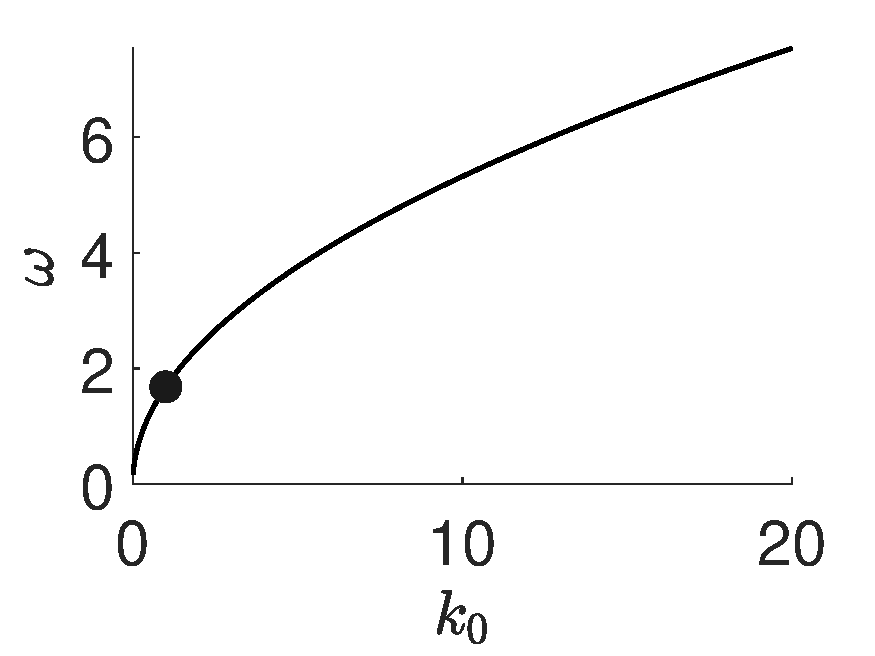
\includegraphics[width=.45\textwidth]{zero_return_shear}
\caption{\small Plot of the zero set $u^{L}_{p}(k_{0},\omega)=0$.  The dot denotes the point $(k_{0},\omega)=(1,1.6818)$.}
\label{fig:zerodriftk0}
\end{figure}

At this point, in order to properly couple our mean surface formulation to the bulk GLM formulation described above, we then require
\[
\left.\bar{{\bf u}}^{L}\right|_{\tilde{z}=\epsilon \bar{\eta}^{L}} = \bar{{\bf u}}^{L}_{s}(\tilde{x},t).
\]
Thus, we then find the integration constant $\tilde{C}(\xi,\tau)$ in the formula for the horizontal LDV $\bar{u}^{L}_{2}$ to be 
\[
\tilde{C}(\xi,\tau) = 2k_{0}\omega\left(-s + \frac{\omega}{\Omega} \right)|\eta_{1}(\xi,\tau)|^{2} + \omega \eta_{0}(\xi,\tau).
\]
Thus, we can find $\bar{u}_{2}^{L}$ as
\begin{multline*}
\bar{u}^{L}_{2}(\xi,\tau,z) = 2k_{0}\omega\left(-s + \frac{\omega}{\Omega} \right)|\eta_{1}(\xi,\tau)|^{2} + \omega \eta_{0}(\xi,\tau) \\
\frac{2\Omega^{2} }{c_{p}-\omega z}\left( 2 + \frac{3\omega}{|k_{0}|(c_{p}-\omega z)}+\frac{2\omega^{2}}{k_{0}^{2}(c_{p}-\omega z)^{2}}\right)|\eta_{1}(\xi,\tau)|^{2} e^{2|k_{0}|z}.
\end{multline*}
We note that if we take the vorticity $\omega=0$, we then get for a left-traveling wave
\[
\bar{u}^{L}_{2}(\xi,\tau,z) = -4k_{0}\Omega|\eta_{1}(\xi,\tau)|^{2}e^{2|k_{0}|z}
\]
Thus, at zero vorticity, we recreate the classic result for the Stokes drift in an irrotational fluid; see \cite{longuet}.  Likewise, even in the case of zero vorticity, we see the impact of the slowly varying envelope introduced by the NLS equation in the need to solve the, in part, slow-variable dependent FMEs, which allows for a more complex relationship between $\bar{{\bf u}}^{L}_{2}$ and the pseudomomentum; see \cite{buhler} for further discussion of this issue.  We likewise note that it is in \cite{buhler} that one sees a clear program for determining $\bar{{\bf u}}^{L}$ via the vorticity and divergence equations we used above in the FMEs.  Aside from computations not appearing in \cite{buhler}, the novel contribution presented herein was in connecting the FMEs to the lifted surface equations, thereby allowing for the connection of the bulk mean velocity to an unambiguously averaged surface result, and allowing for a continuously defined LDV.  

Following \cite{andrews}, we define the Stokes drift of a quantity, say $\bar{\varphi}^{S}$ to be 
\[
\bar{\varphi}^{S} = \bar{\varphi}^{L} - \bar{\varphi}.
\]

Thus, if we average the fluid velocity in the bulk of the fluid, Equations \eqref{phixexp} and \eqref{phizexp} show that the bulk Eularian mean horizontal velocity is given by $\bar{u}(\xi,\tau,z)$ where
\[
\bar{u}(\xi,\tau,z) = \omega z + \mathcal{O}(\epsilon^{3}).
\]
Thus, in the bulk, the horiontal SVD, say $\bar{u}^{S}_{2}(\xi,\tau,z) = \bar{u}^{L}_{2}(\xi,\tau,z)$.  We emphasize that $z$ is a mean coordinate, and thus we do not evaluate the LVD or SVD at the free surface $z=\epsilon \eta(x,t)$, but instead at the lifted surface $\tilde{z}=\epsilon \bar{\eta}^{L}$.  Near the lifted free surface, by removing the Eularian mean term $\omega \eta_{0}$, we have that the surface SDV in the horizontal direction, say $\bar{u}^{S}_{s}$ is 
\begin{equation}
\bar{u}^{S}_{s}(\xi,\tau) = -2\epsilon^{2}k_{0}\Omega\left(1 + \left(1-\frac{s\omega}{\Omega} \right)^{2}\right)|\eta_{1}(\xi,\tau)|^{2}.
\label{surfSDV}
\end{equation}
Note, this multi-part definition for the SDV reflects the intricacies of averaging around a freely evolving surface.  This explains our privileging of the LDV over the SDV.  Our result then provides support for the phenomenological choices of how the SDV of a plane-wave varies in depth made in \cite{breivik}.  There, the classic formula for the SDV was modified by multiplying it by terms like $1/(1+\tilde{c}z)$, where $\tilde{c}$ was then chosen to improve agreements with observed data.  Our result provides a physical motivation for the appearance of such terms.  However, while we can put forth a physical mechanism, whether unresolved shear currents near the surface are truly responsible for disagreements between theory and observation is a matter for future work.

\subsubsection*{The Surface SDV for Modulated Surface Waves}
The surface SDV in Equation \eqref{surfSDV} for the Jacobi elliptic function solutions with $\beta=1$ is given by
\[
\bar{u}^{S}_{s}(\xi,\tau) = -4\epsilon^{2}\kappa^{2}k_{0}\Omega \left|\frac{\alpha_{d}}{\alpha_{nl}}\right| \left(1 + \left(1 - \frac{s\omega}{\Omega} \right)^{2} \right)\phi(\xi;\kappa),
\]
where
\[
\phi(\xi;\kappa) = \left\{\ba{rl} \mbox{cn}^2(\xi;\kappa), & \alpha_{d}/\alpha_{nl}>0, \\  \mbox{sn}^2(\xi;\kappa), & \alpha_{d}/\alpha_{nl}<0,\ea \right.
\]
where $\xi$ is defined in Equation (\ref{xidef}).  Defining the parameter
\[
\tilde{u}^{S}(k_{0},\omega) = -4 k_{0}\Omega(k_{0},\omega) \left|\frac{\alpha_{d}(k_{0},\omega)}{\alpha_{nl}(k_{0},\omega)}\right|\left(1 + \left(1 - \frac{s\omega}{\Omega(k_{0},\omega)} \right)^{2} \right),
\]
and choosing the positive branch of the dispersion relationship, Figure \ref{fig:sdriftmag_sign} shows that this term exhibits a wide variation in magnitude.  The curves along which the largest magnitudes are seen correspond to the level set $\alpha_{nl}(k_{0},\omega)=0$.  Thus, for the class of Jacobi elliptic solutions, there appears to be a kind of nonlinear resonance between the shear current and the carrier wave.  We point out that along this curve though, the assumptions we used to derive the NLS equation are no longer valid.  Therefore, more work should be done to better elucidate the affiliated dynamics associated with parameter choices defining said curve.  Throughout the remainder of this paper, we choose parameter values that do not place us too close to the zero set of $\alpha_{nl}(k_{0},\omega)=0$.
\begin{figure}
\centering
\begin{tabular}{c}
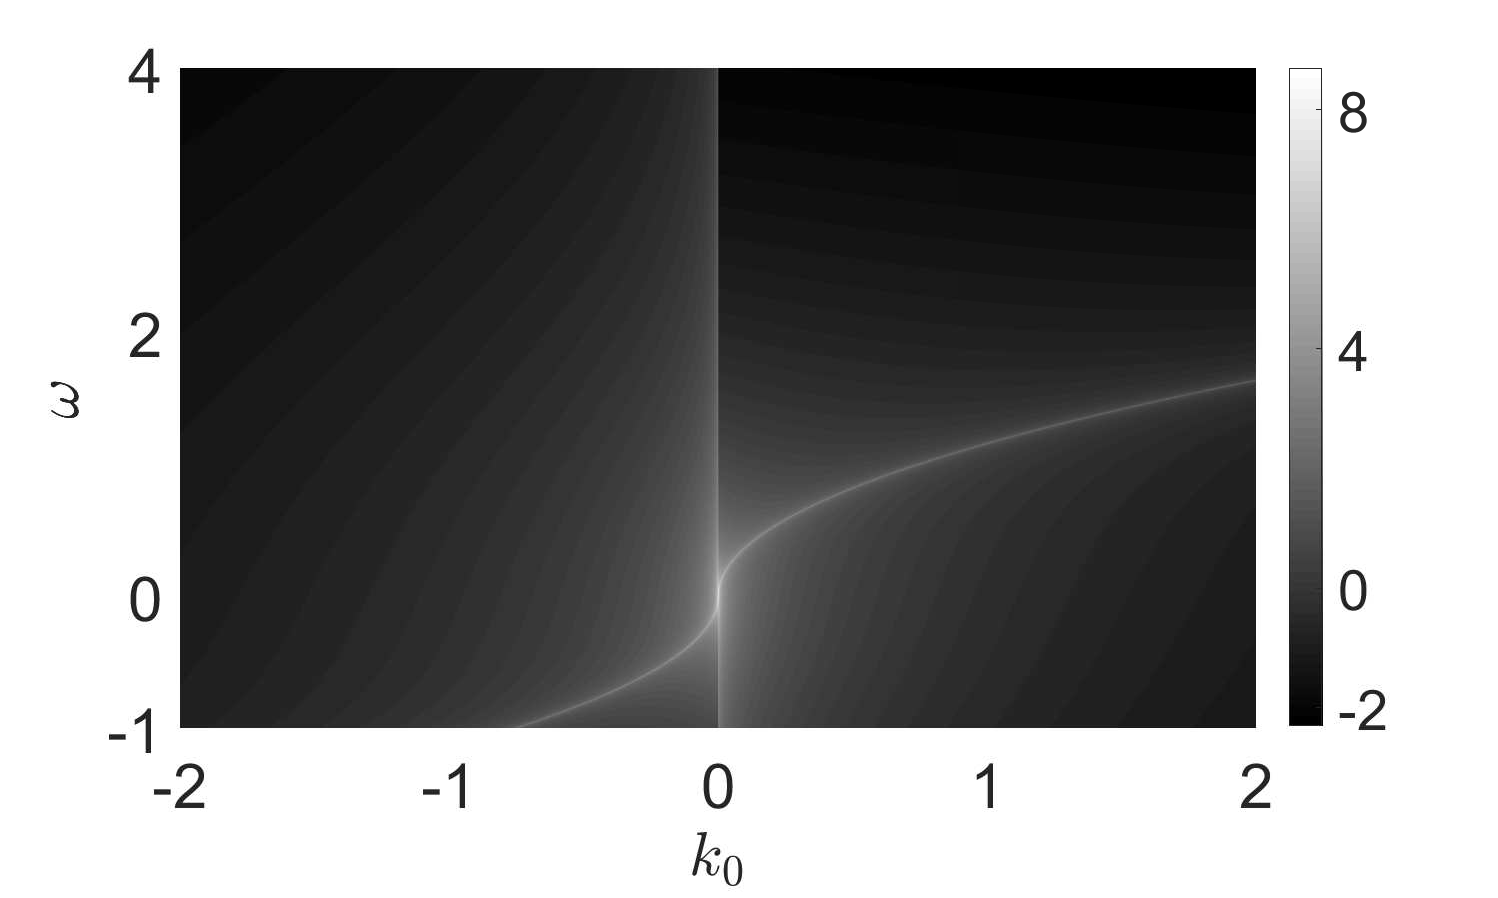
\includegraphics[width=.55\textwidth]{us_magnitude}
\end{tabular}
\caption{\small Log plot of the surface SDV parameter $\tilde{u}^{S}(k_{0},\omega)$.  The curves along which $\tilde{u}^{S}(k_{0},\omega)=0$ mirror the transitions between MI stable and unstable regions seen in Figure \ref{fig:miplot}.  The surface SDV is most augmented near the curves corresponding to $\alpha_{nl}(k_{0},\omega)=0$.  }
\label{fig:sdriftmag_sign}
\end{figure}

To get a more detailed understanding of how the surface SDV depends on the shear current strength, we choose $k_{0}=1$ and use the positive branch of the dispersion relationship.  Figure \ref{fig:stksdrfcomp} contains plots of $\tilde{u}^{S}(1,\omega)$ for $-1\leq \omega\leq 4$, $-1\leq \omega \leq 1.1$, and $1.2\le\omega\le4$.  We choose these particular ranges of shear values to in particular examine the behavior of $\tilde{u}^{S}$ around the resonance curve seen in Figure \ref{fig:sdriftmag_sign}.  The singularity seen in Figure \ref{fig:stksdrfcomp} (a) corresponds to the value $\omega$ such that $\alpha_{nl}(1;\omega)=0$, namely $\omega\approx1.1550$.  Figure \ref{fig:stksdrfcomp} (b) shows the focusing side and that increasing the shear strength increases the Stokes drift velocity.  Figure \ref{fig:stksdrfcomp} (c) shows that this relationship is reversed on the defocusing side.
\begin{figure}
\centering
\begin{tabular}{ccc}
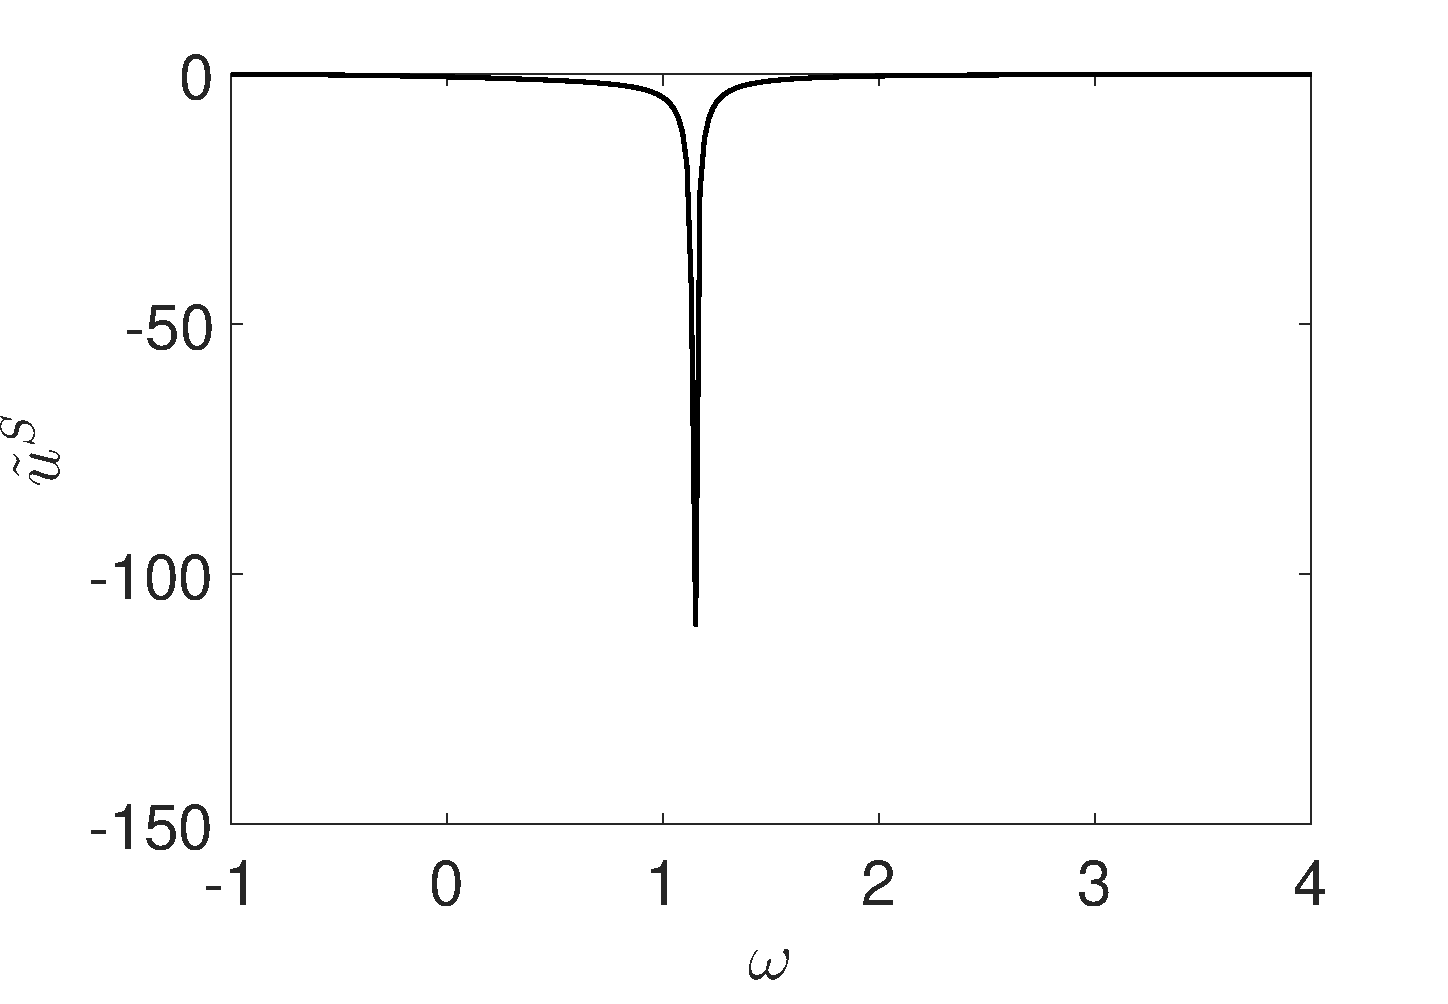
\includegraphics[width=.32\textwidth]{us_wide_range} & 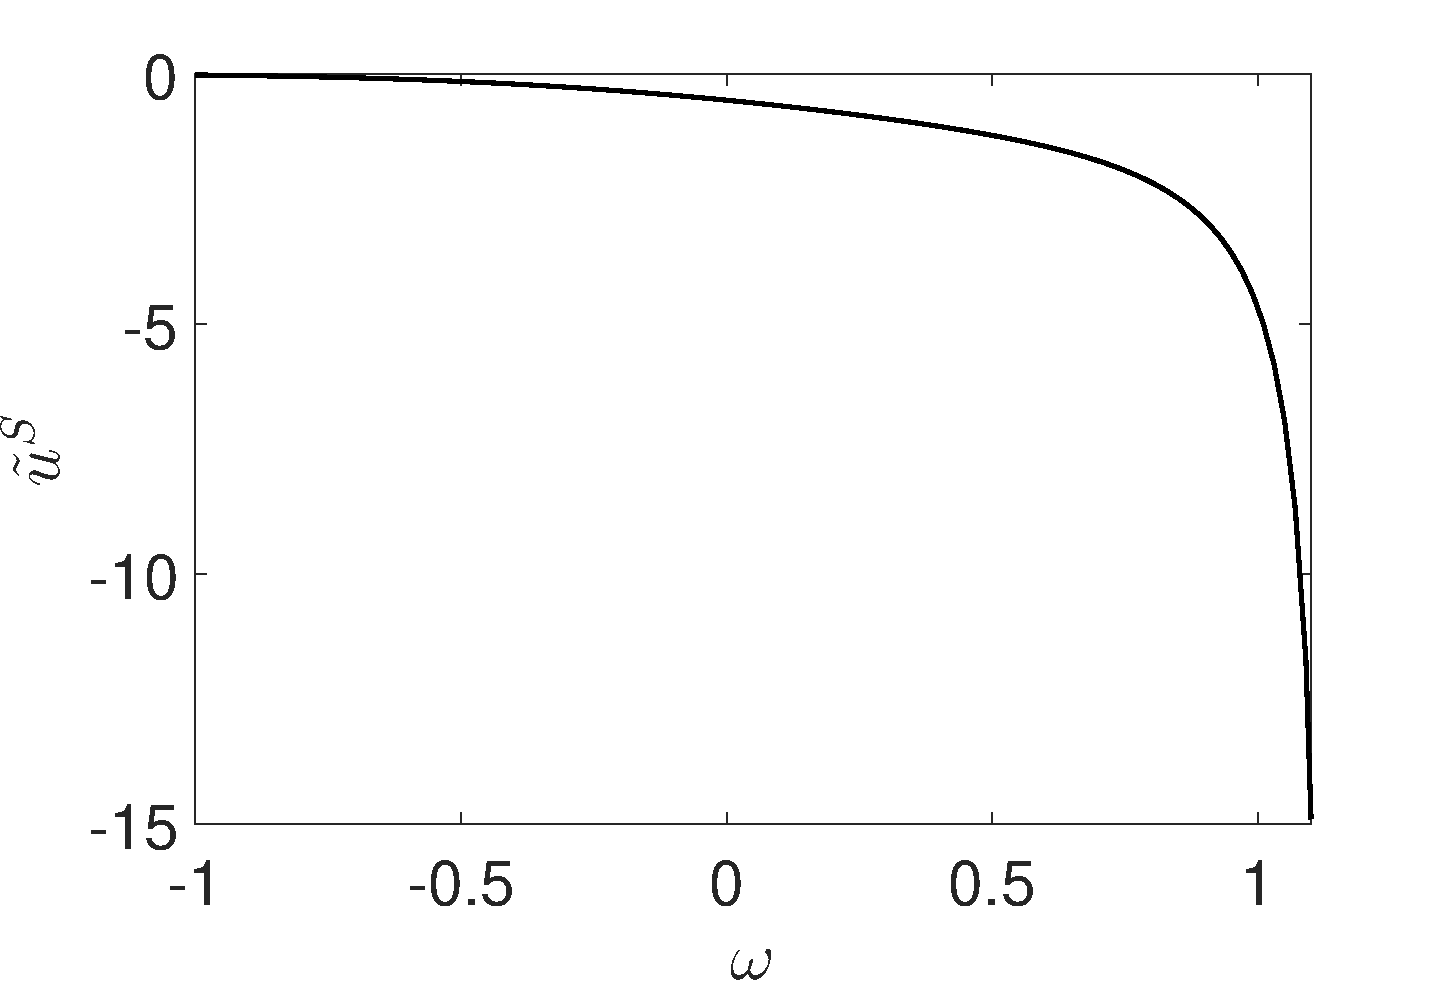
\includegraphics[width=.32\textwidth]{us_n1_to_1pt1} & 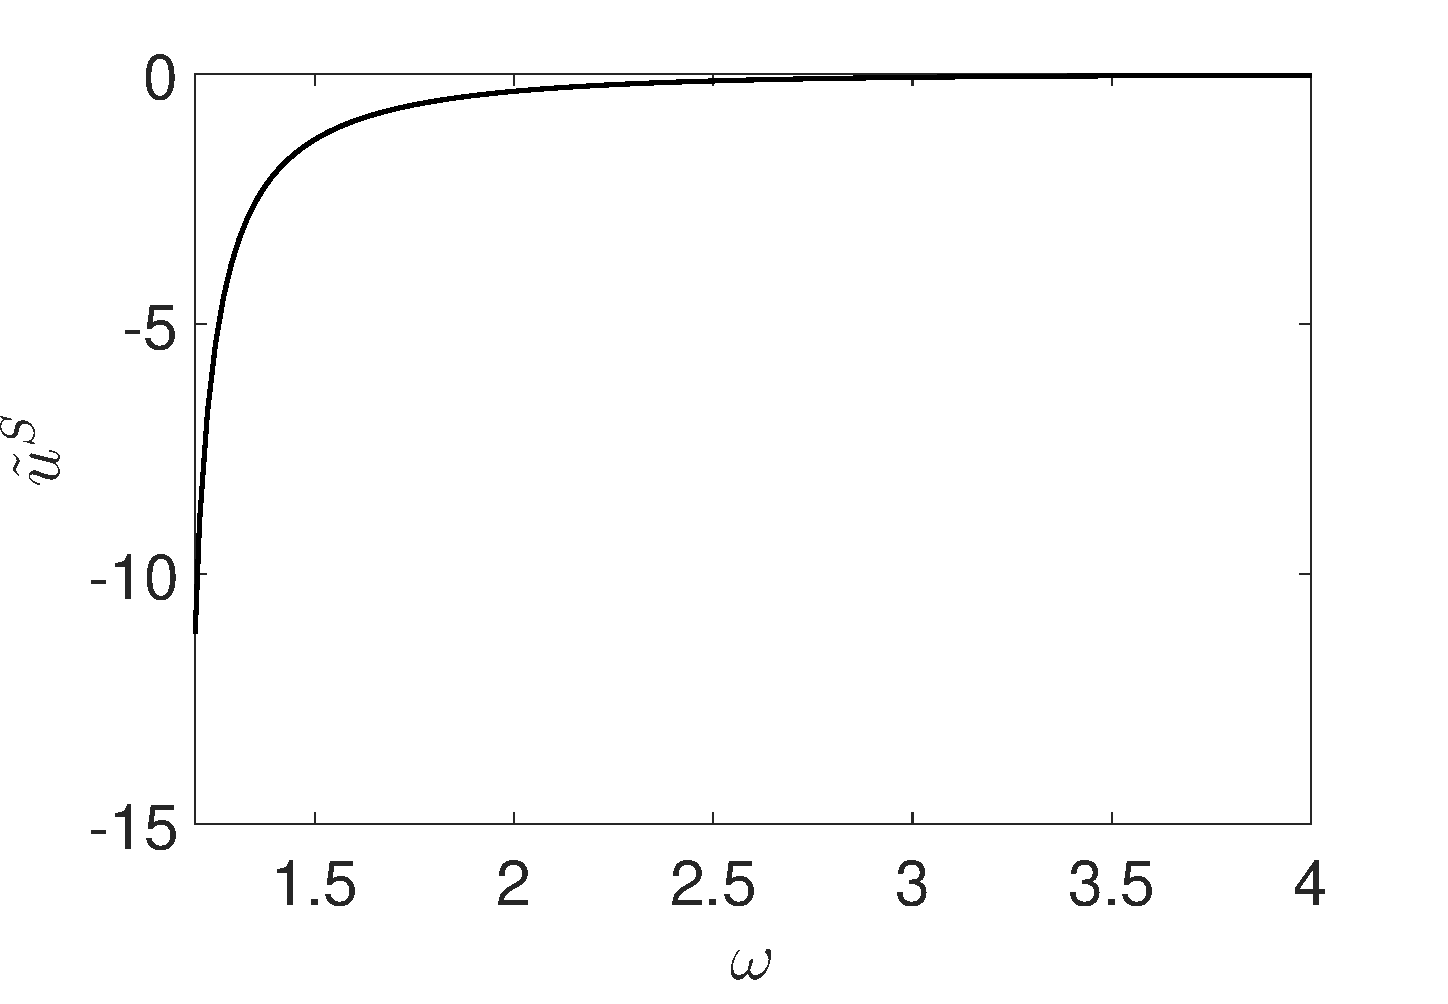
\includegraphics[width=.32\textwidth]{us_1pt2_to_4}\\
(a) & (b) & (c)
\end{tabular}
\caption{\small Plots of $\tilde{u}^{S}(1,\omega)$ for $-1\leq \omega \leq 4$ (a), $-1\leq \omega \leq 1.12$ (b), and $1.17\leq \omega \leq 4$ (c).  Note, $\alpha_{nl}(1;1.1550)=0$.  This shows that the magnitude of the SDV increases with increasing shear on the focusing side of the singularity (b), and decreases with increasing shear on the defocusing side (c).}
\label{fig:stksdrfcomp}
\end{figure}

\subsection{Flow Near the Depth $z_{c}$}
Again the depth $z_{c}=c_{p}/\omega$ is the depth at which our approximations to the mean particle path fluctuations in Equations \eqref{meanfc1} and \eqref{meanfc2} are no longer valid.  Taking $k_{0}\omega >0$ so that $-\infty<z_{c}<-1$, it is illuminating to attempt to examine particle paths near this depth.  To do this, we look at the special case of a plane wave solution to the NLS equation, so that we can readily write 
\begin{align*}
\dot{x} = & \omega z - 2\epsilon s\Omega A e^{|k_{0}|z}\cos(\tilde{\theta}) + \mathcal{O}(\epsilon^{2})\\
\dot{z} = & -2\epsilon\Omega A e^{|k_{0}|z}\sin(\tilde{\theta}) + \mathcal{O}(\epsilon^{2}),
\end{align*}
where $\tilde{\theta} = \theta + \epsilon^{2}\alpha_{nl}A^{2}t$.  At this order, we can rewrite this system as 
\begin{align*}
\dot{\tilde{\theta}} = & \Omega+k_{0}\omega z - 2\epsilon |k_{0}|\Omega A e^{|k_{0}|z}\cos(\tilde{\theta}) + \mathcal{O}(\epsilon^{2}),\\
\dot{z} = & -2\epsilon\Omega A e^{|k_{0}|z}\sin(\tilde{\theta}) + \mathcal{O}(\epsilon^{2}),
\end{align*}
which to leading order is seen to have the Hamiltonian $H(\tilde{\theta},z)$ where
\[
H(\tilde{\theta},z) = \Omega z + \frac{k_{0}\omega z^{2}}{2} - 2\epsilon\Omega A e^{|k_{0}|z}\cos(\tilde{\theta}).
\]
This has critical points at 
\[
\tilde{\theta}=n \pi, ~ z = z_{c} - \epsilon\frac{2c_{p} e^{|k_{0}|z_{c}}}{\omega} (-1)^{n} + \mathcal{O}(\epsilon^{2}),
\]
with even $n$ corresponding to centers and odd $n$ to saddles.  This result then is a good indication for the presence of `cats-eye' patterns around the depth $z_{c}$, a result echoing the works of \cite{simmen,dasilva,wahlen2} and \cite{nachbin} among many other authors.  This presents an interesting matching problem with regards to finding uniform approximations to the LDV.  This however is a question beyond the scope of the present paper.
%%%%%%%%%%%%%%%%%%%%%%%%%%%%%%%%%%%%%%%%%%%%%%%%%%%%%%%%%%%%%%%%%%%%%%%%%%%%%%%%%%%
%%%%%%%%%%%%%%%%%%%%%%%%%%%%%%%%%%%%%%%%%%%%%%%%%%%%%%%%%%%%%%%%%%%%%%%%%%%%%%%%%%%
\section{Numerical Results}
In order to determine particle paths, say $(x(t),z(t))$, in general, the system in Equation (\ref{system}) must be solved.  However, we focus on determining particle paths at the surface. Thus, letting $\tilde{\eta}$ denote the truncation of Equation \eqref{nlssurfexp} up to and including $\mathcal{O}(\epsilon)$ terms, we approximate the vertical component of the path via the restriction  
\[
z(t) = \epsilon \tilde{\eta}(x(t),t).
\]
We then can readily find the scalar equation for the horizontal coordinate $x(t)$ to be
\[
\dot{x} = \epsilon\omega\tilde{\eta}(x,t) + \epsilon \tilde{\phi}_{x}(x,\epsilon\tilde{\eta}(x,t),t) 
\]
where the potential $\tilde{\phi}_{x}$ is found using Equation \eqref{phixexp}.  However, since the NLS solutions are in terms of the coordinates $\xi$ and $\tau$, we rewrite the above equation in these coordinates so that we have 
\begin{equation}
\frac{d \xi}{d\tau} =  \frac{c_{g}}{\epsilon} + \omega\tilde{\eta}\left(\xi,\tau\right) + \tilde{\phi}_{x}(\xi,\epsilon\tilde{\eta}),
\label{pathode}
\end{equation}
\[
\xi(0)=\xi_0.
\]
We use a fourth-order Runge-Kutta (RK4) scheme with a time step of $\delta \tau = 5\times10^{-4}$ to solve this initial-value problem.  To solve for the evolution of $\eta_{1}(\xi,\tau)$, we use a pseudo-spectral scheme with $1024$ modes to discretize the VD Equation in space thereby allowing it to be coupled to the RK4 scheme used in Equation \eqref{pathode}. We can then determine $\eta_{1}(\xi,\tau)$ up to and including $\mathcal{O}(\epsilon)$ effects on a $\mathcal{O}(1/\epsilon^{2})$ timescale.  We use the Jacobi elliptic or plane wave solutions to the NLS equation as an initial condition to the VD equation.  By using the VD equation, we see that on the $\mathcal{O}(1)$ in $\tau$, or $\mathcal{O}(1/\epsilon^{2})$ in $t$, time scale of the NLS equation, we anticipate that the error from truncation in Equation \eqref{pathode} should be at worst $\mathcal{O}(\epsilon^{2})$ in $\xi$ and thus at worst $\mathcal{O}(\epsilon)$ in $x(t)$.  Per our restriction on $z(t)$, this implies that at worst we should anticipate errors of $\mathcal{O}(\epsilon^{2})$ on the longer time scales corresponding to the nonlinear effects.  

For the Jacobi elliptic function solutions, we chose the initial tracer position to be
\[
\xi(0) = \frac{K(\kappa)}{128}, ~ z(0) = \epsilon \tilde{\eta}(\xi(0),0),
\]
where $K(\kappa)$ is the complete elliptic integral of the first kind and $\tilde{\eta}$ is defined by Equation \eqref{nlssurfexp}.  For the plane-wave solutions, we chose $\xi_{0}=10/128$ so the initial positions are comparable across the different classes of solutions.  We take the positive branch of the dispersion relationship, which implies that $k_{0}>0$ corresponds to a left-moving-carrier wave.  We choose $k_{0}=1$ for the plane-wave solutions.  In the case of the Jacobi elliptic solutions to the NLS equation, we choose the integer $m$ to be
\[
m = \left\lfloor \frac{2K(\kappa)}{\pi \epsilon}\right\rfloor,
\]
so that, using Equation \eqref{jacwavnum}, $k_{0}\approx 1$.  In practice, $k_{0}\approx0.98$ or $0.99$.  The results for the tracer position in physical coordinates, $(x(t),z(t))$, are found using the transformations
\[
x(t) = \frac{\xi(\tau)}{\epsilon}-\frac{c_{g}\tau}{\epsilon^{2}}, ~~~~ t = \frac{\tau}{\epsilon^{2}}.
\]
Fourier transforms and their inverses are computed numerically using the fast Fourier transform.

Finally, the expansions in \eqref{phixexp} and \eqref{phizexp}, and the associated approximations in \eqref{roeqx} and \eqref{roeqz}, show that the strength of the velocity field is largely determined by the magnitude of the solution to the NLS equation which is the leading order approximation to $\eta_{1}$.  In the case of the Jacobi elliptic function solutions, controlling for the elliptic modulus $\kappa$, the term $\sqrt{2|\alpha_{d}/\alpha_{nl}|}$ is the most significant contribution to the magnitude of $\eta_{1}$ since we have fixed $\beta=1$; see Equations \eqref{cnsolns} and \eqref{snsolns}.  Figure \ref{fig:ampcomps} contains plots of $\sqrt{2|\alpha_{d}/\alpha_{nl}|}$ versus $\omega$ for $k_0=1$.  Note, we take $\omega = \mathcal{O}(1)$ to be consistent with our derivation of the VD equation.  
\begin{figure}
\centering
\begin{tabular}{ccc}
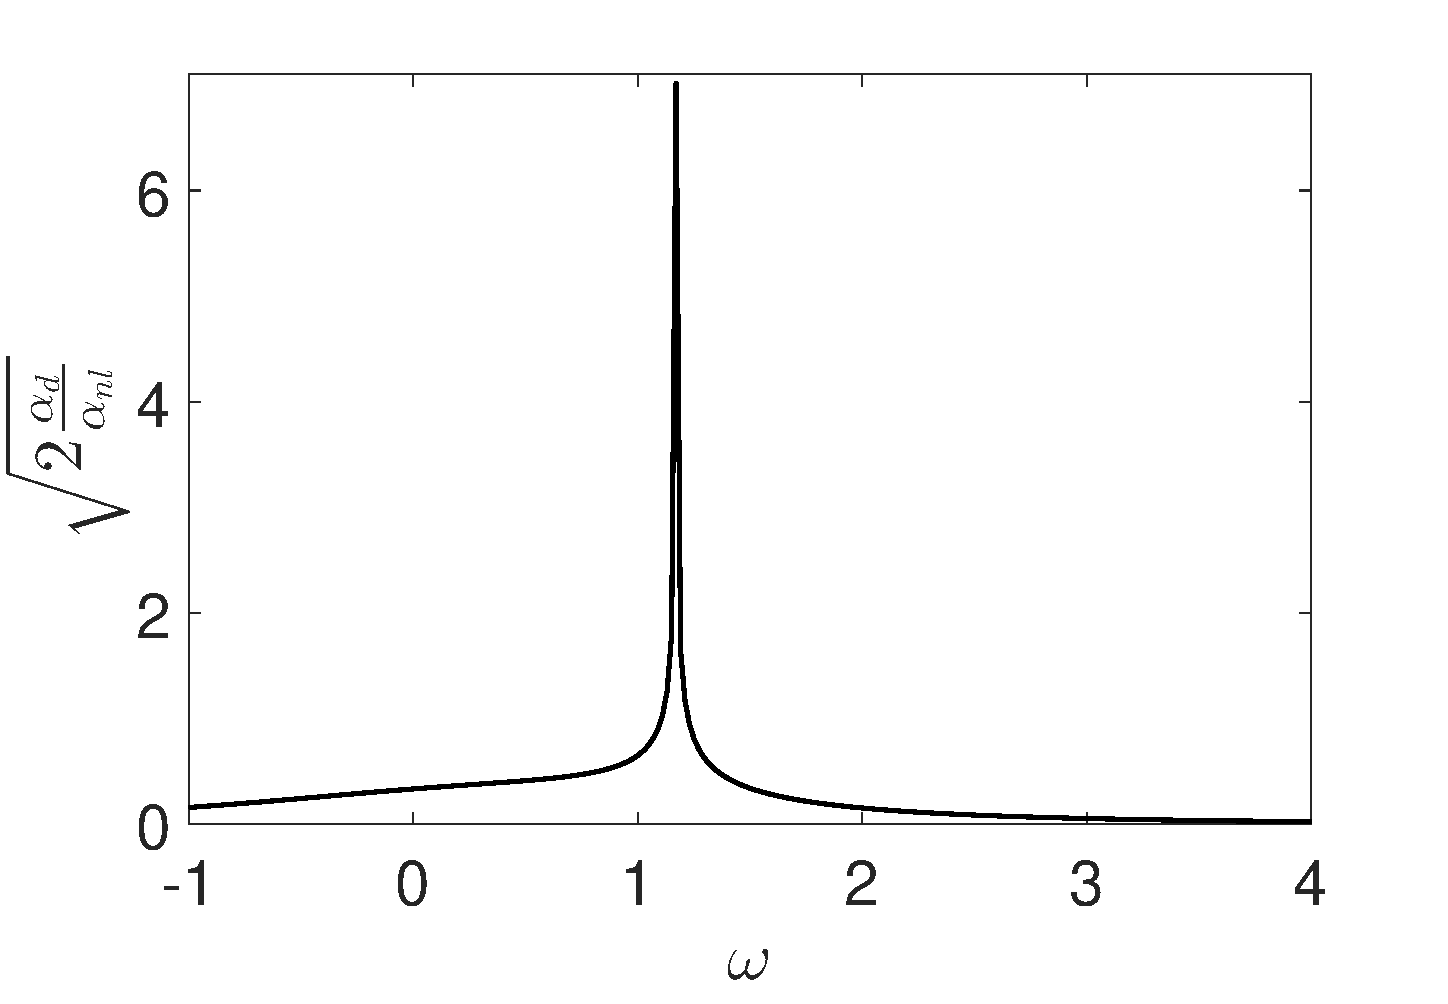
\includegraphics[width=.32\textwidth]{amp_factor_k0_1_wide_range} & 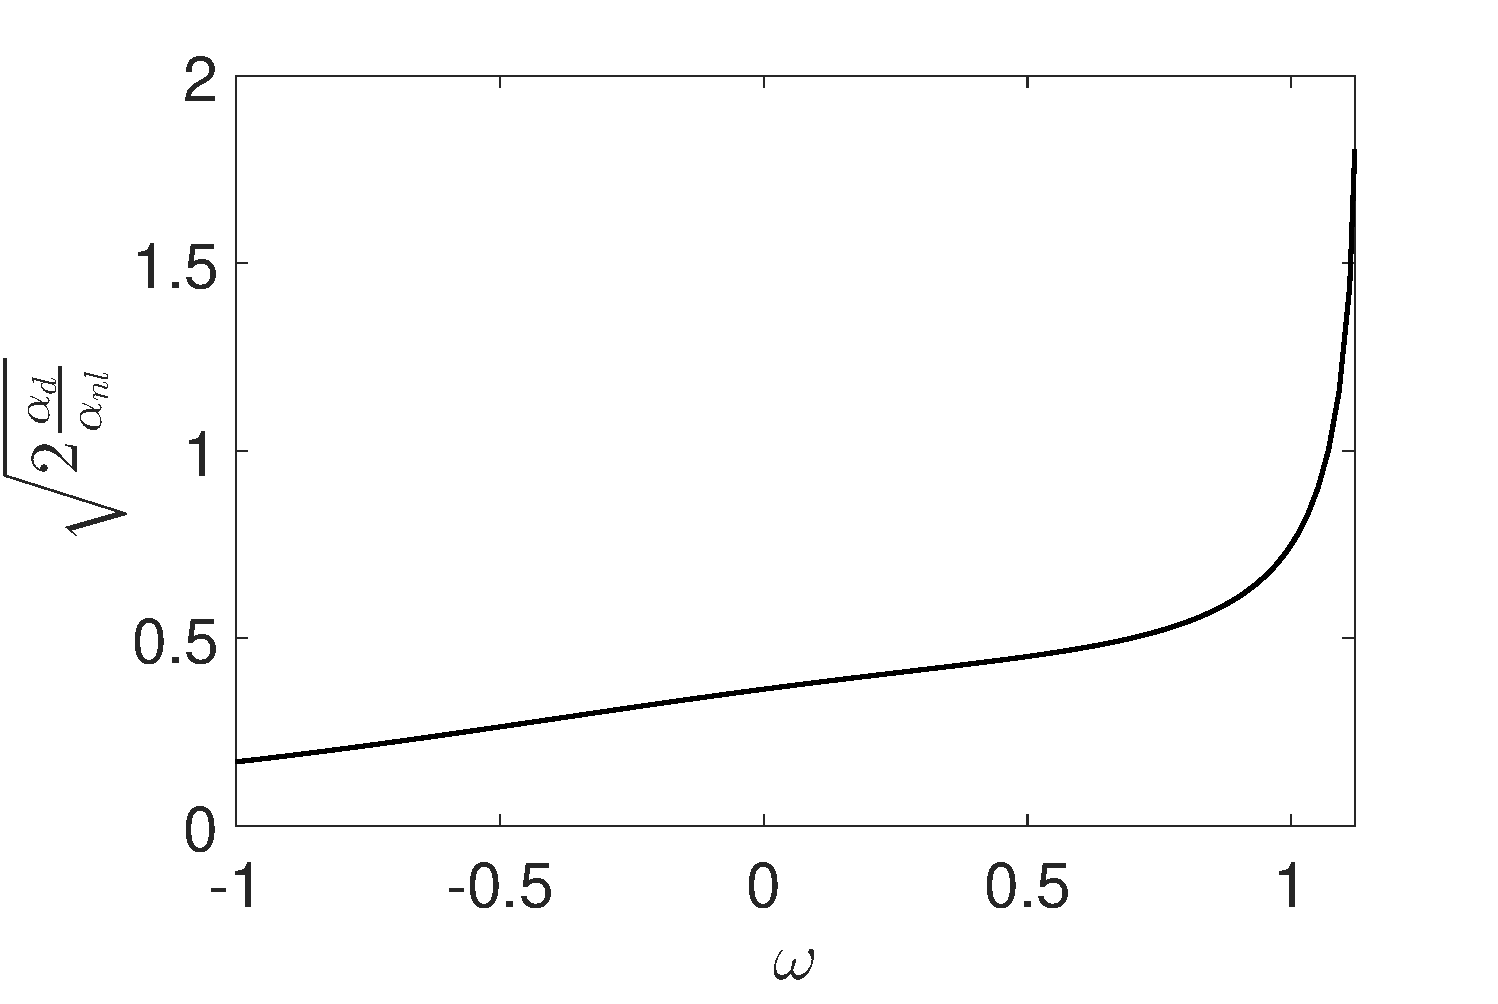
\includegraphics[width=.32\textwidth]{amp_factor_k0_1_n1_to_1pt12} & 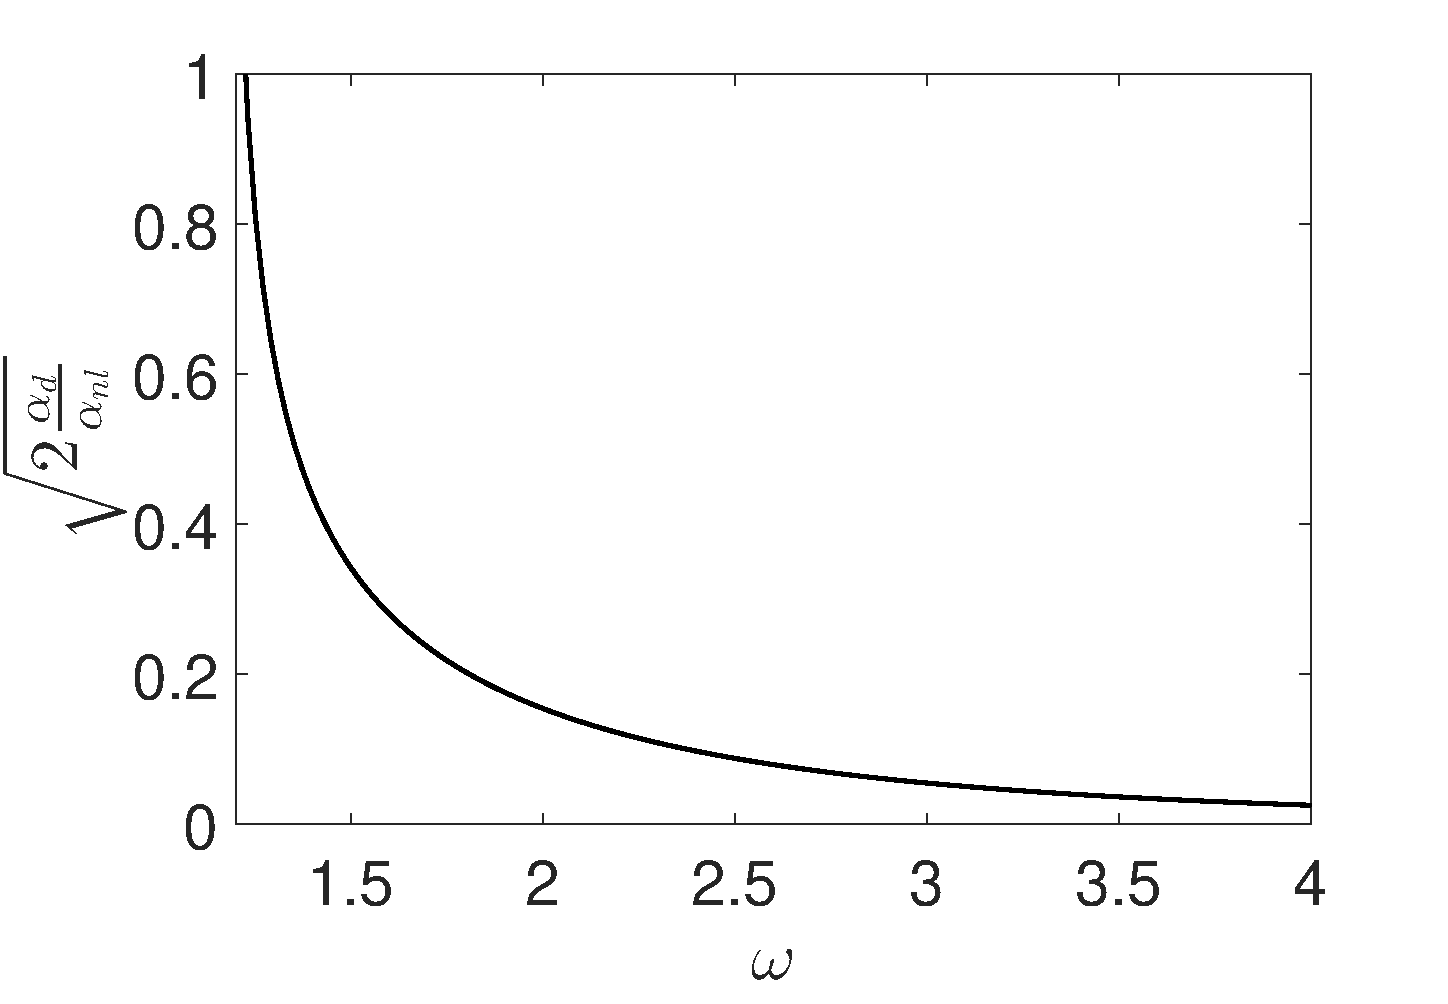
\includegraphics[width=.32\textwidth]{amp_factor_k0_1_1pt2_to_4}\\
(a) & (b) & (c)
\end{tabular}
\caption{\small Strength of the surface velocity as measured via plots of $\sqrt{2|\alpha_{d}/\alpha_{nl}|}$ for $k_{0}=1$ for $-1\leq \omega \leq 4$ (a), $-1\leq \omega \leq 1.12$ (b), and $1.17\leq \omega \leq 4$ (c).  Increasing shear increases the velocity on the focusing side, and decreases it on the defocusing side.}
\label{fig:ampcomps}
\end{figure}
In the focusing case, increasing the magnitude of the Jacobi elliptic function solutions corresponds to increasing the shear strength.  In the defocusing case, decreasing the magnitude of the Jacobi elliptic function solutions corresponds to increasing the shear strength.  These two statements are justified by the similarities of Figures \ref{fig:ampcomps} (b) and (c) and \ref{fig:stksdrfcomp} (b) and (c).  Therefore, relatively large amplitude solutions inducing strong fluid particle drift is to be expected near the resonance curve.
%%%%%%%%%%%%%%%%%%%%%%%%%%%%%%%%%%%%%%%%%%%%%%%%%%%%%%%%%%%%%%%%%%%%%%%%%%%%%%%%%%%
\subsection{Focusing Case}

Using the solution given in equation \eqref{cnsolns} with $k_0\approx1$ ensures that $\omega = 0$ and $\omega=\pm 1$ are in the focusing regime.   Figure \ref{fig:foc_kap_pt5} shows the paths of particles as well as there mean paths for three values of $\omega$ found by setting $\epsilon=0.1$, $\kappa=0.5$, and solving the dynamical system for the particle and mean paths up to time $t=1/\epsilon^{2}$.  The carrier profile is propagating to the left in this situation.  Therefore, if $\omega=1.12$, then the shear current is counter-propagating at the surface with respect to the carrier wave while if $\omega=-1$, the current is co-propagating.  The counter-propagating current significantly enhances the leftward horizontal motion of a tracer along the surface as seen by comparing Figures \ref{fig:foc_kap_pt5}(b) and (c) with (a).  This can be explained by comparing the values of the SDV and the LDV parameters
\[
\begin{array}{lcl}
\tilde{u}^{S}(1,0) = -0.5222, & & \tilde{u}^{L}(1,0) = -0.5222,\\
\tilde{u}^{S}(1,1.12) = -10.7373,& & \tilde{u}^{L}(1,1.12) = -5.2195,\\
\tilde{u}^{S}(1,-1) = -0.2836, & & \tilde{u}^{L}(1,-1) = -0.1636,
\end{array}
\]
where the parameter $\tilde{u}^{L}$ is defined to be
\[
\tilde{u}^{L}(k_{0},\omega) = 2\left|\frac{\alpha_{d}(k_{0},\omega)}{\alpha_{nl}(k_{0},\omega)}\right|u^{L}_{p}(k_{0},\omega).
\]
Note that for the Jacobi elliptic solutions and controlling for $\kappa$ and $\beta$, this will be the most significant contribution to the magnitude of the LDV.  This demonstrates why the counter-propagating current so enhances the leftward drift since the LDV parameter is an order of magnitude larger than in the other cases.    Further, it demonstrates why the co-propagating current, i.e. $\omega=-1$, reduces the horizontal displacement of the surface particle.  This is somewhat surprising as one might intuitively imagine that the co-propagating shear would enhance the particle drift, especially in comparison to the zero vorticity case.  However, we have effectively shown that nonlinearity makes the surface/current interaction a more complicated one than one might at first suspect.
\begin{figure}
\centering
\begin{tabular}{cc}
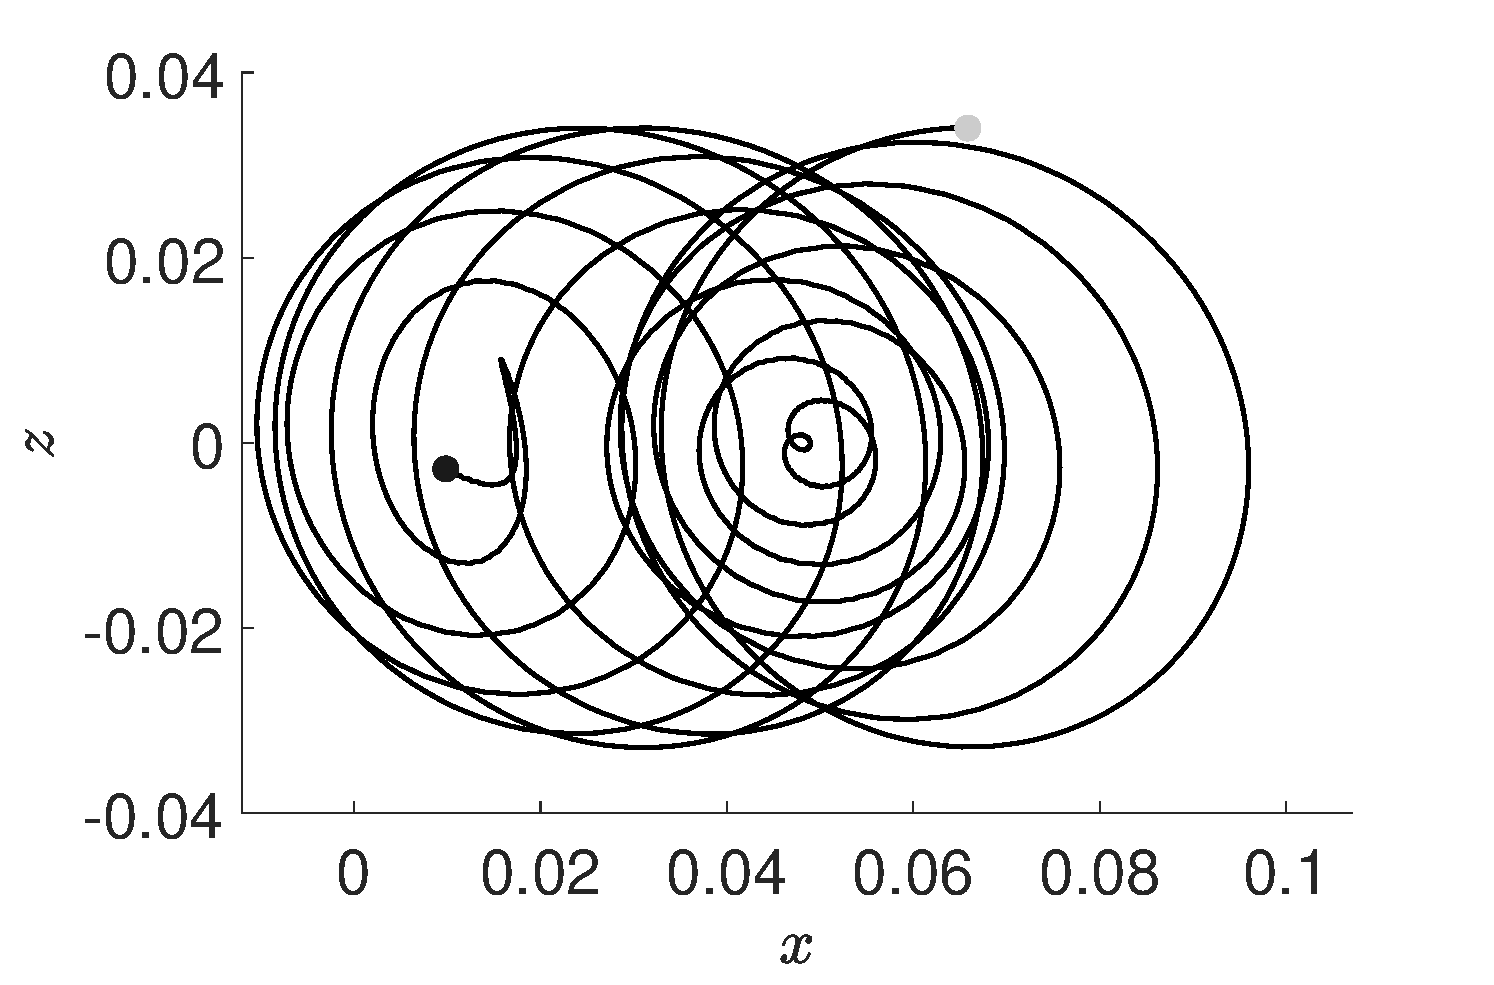
\includegraphics[width=.48\textwidth]{track_ep_pt1_tf_1_w_0_kap_pt5_foc} & 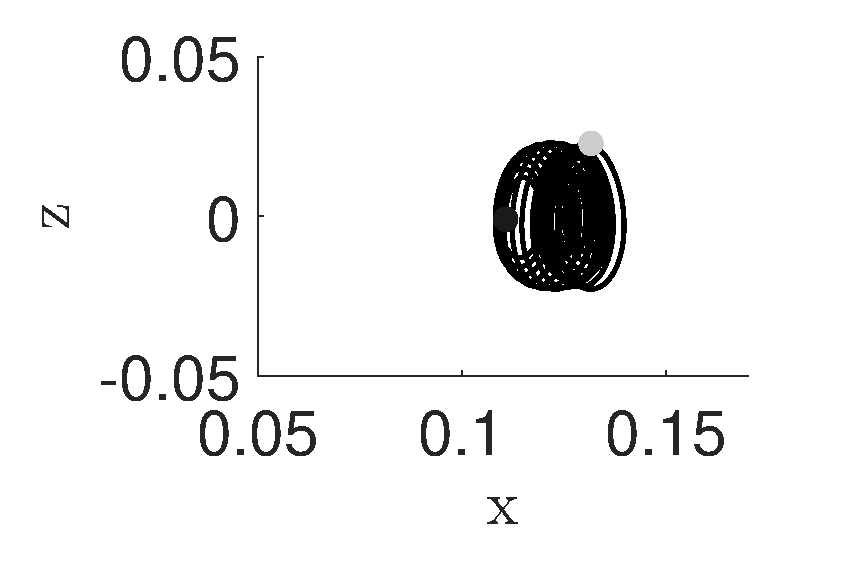
\includegraphics[width=.48\textwidth]{track_ep_pt1_tf_1_w_1_kap_pt5_foc} \\
(a) & (b) \\
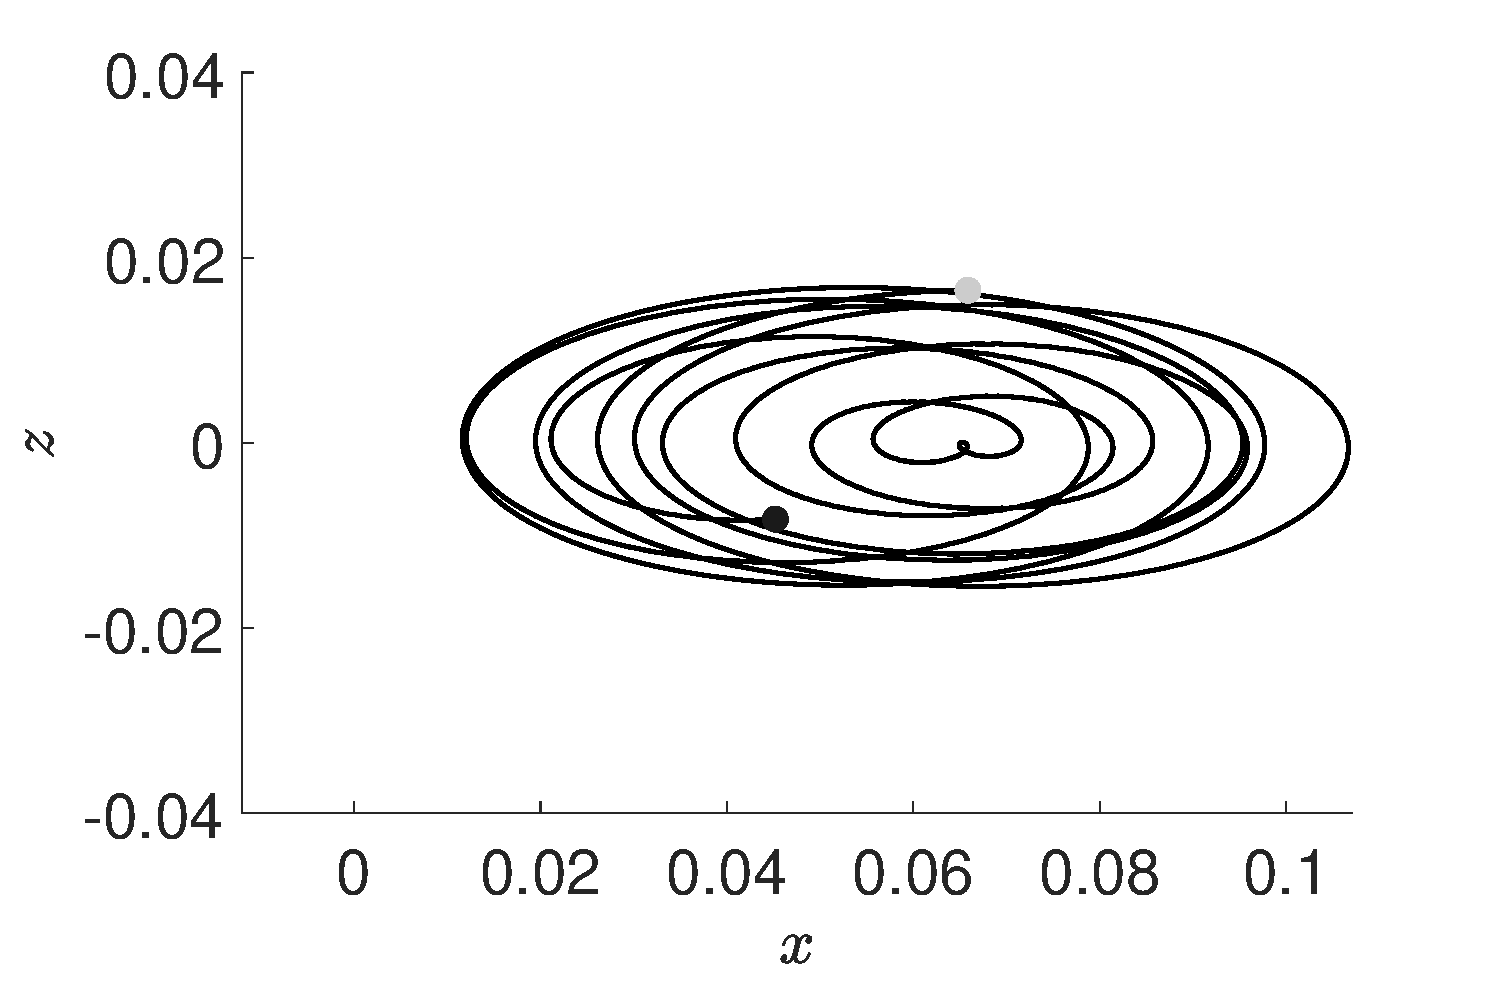
\includegraphics[width=.48\textwidth]{track_ep_pt1_tf_1_w_n1_kap_pt5_foc} & \\
(c) &
\end{tabular}
\caption{\small {\bf Focusing Case} - Plots of particle paths correspond to the solution given in Equation (\ref{cnsolns}) with $\epsilon=0.1$, $\beta=1$, $k_{0}\approx 1$, $\kappa=0.5$, with $\omega=0$ (a), $\omega=1.12$ (b), and $\omega=-1$ (c). The grey dots indicate the starting positions of the tracers while the black dots indicate their final positions.}
\label{fig:foc_kap_pt5}
\end{figure}

Choosing $\kappa=0.99$ shows that similar results hold closer to the solitary wave solution; see Figure \ref{fig:foc_kap_pt99}, though the larger elliptic modulus results in the larger amplitudes and leftward drifts.  In particular, near the solitary wave limit, positive, counter-propagating shear can greatly enhance both the impact of nonlinearity and the transport properties of the waves.
\begin{figure}
\centering
\begin{tabular}{cc}
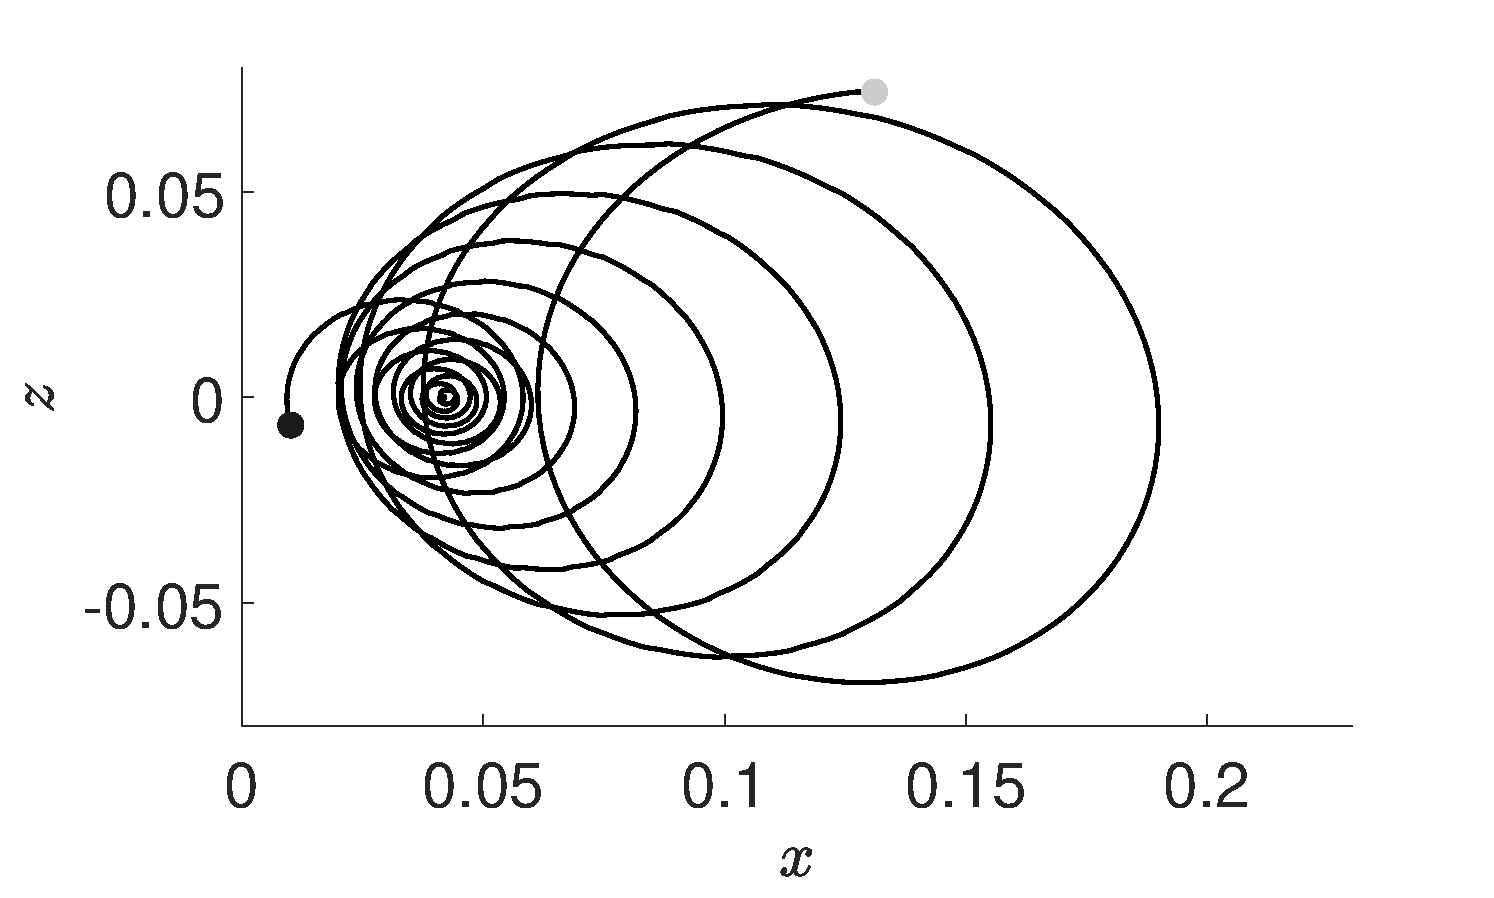
\includegraphics[width=.48\textwidth]{track_ep_pt1_tf_1_w_0_kap_pt99_foc} & 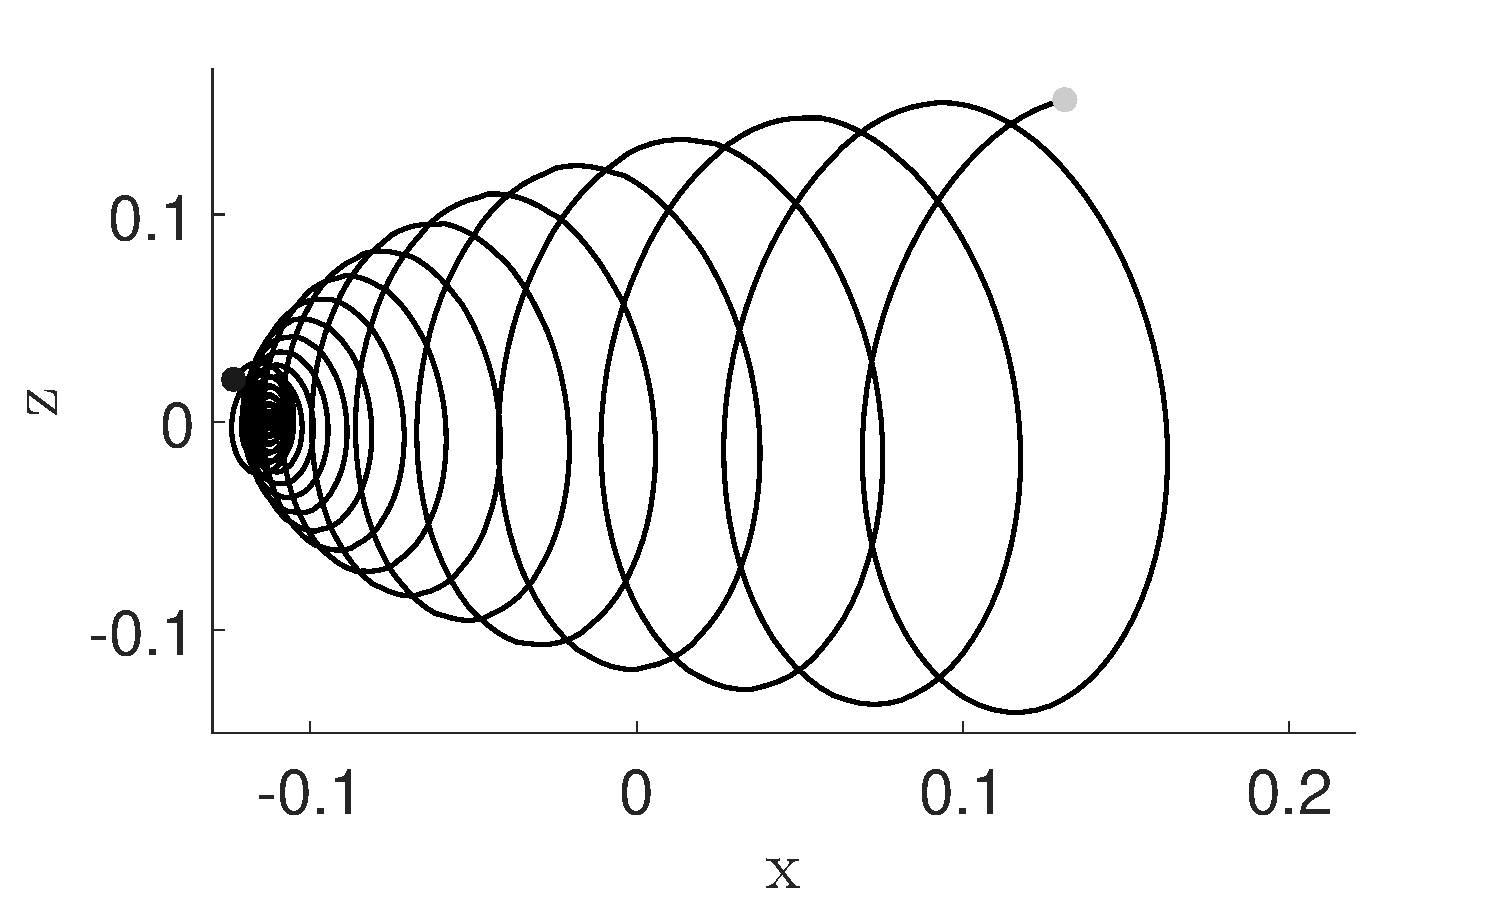
\includegraphics[width=.48\textwidth]{track_ep_pt1_tf_1_w_1_kap_pt99_foc} \\
(a) & (b) \\
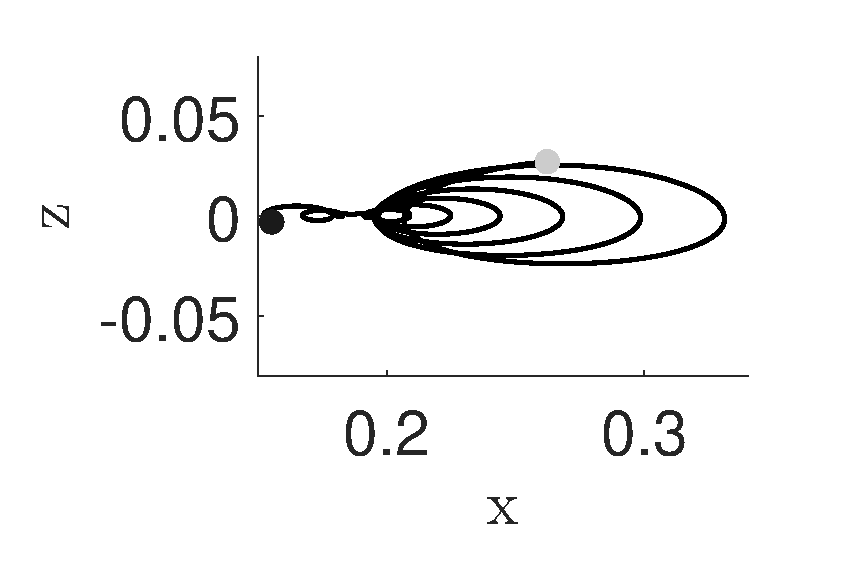
\includegraphics[width=.48\textwidth]{track_ep_pt1_tf_1_w_n1_kap_pt99_foc} & \\
(c) &
\end{tabular}
\caption{\small {\bf Focusing Case} - Plots of particle paths correspond to the solution given in Equation (\ref{cnsolns}) with $\epsilon=0.1$, $\beta=1$, $k_{0}\approx 1$, $\kappa=0.99$, with $\omega=0$ (a), $\omega=1.12$ (b), and $\omega=-1$ (c). The grey dot indicates the starting position of the tracer while the black dot indicates the final position.}
\label{fig:foc_kap_pt99}
\end{figure}

%%%%%%%%%%%%%%%%%%%%%%%%%%%%%%%%%%%%%%%%%%%%%%%%%%%%%%%%%%%%%%%%%%%%%%%%%%%%%%%%%%%
\subsection{Defocusing Case}

For the Jacobi elliptic solutions with $k_{0}\approx 1$, the zero LDV solutions belong in the defocusing case.  Figure \ref{fig:jaczerodrift} shows the impact on surface flow particle paths when $\omega$ is chosen to zero out the LDV.
\begin{figure}
\centering
\begin{tabular}{cc}
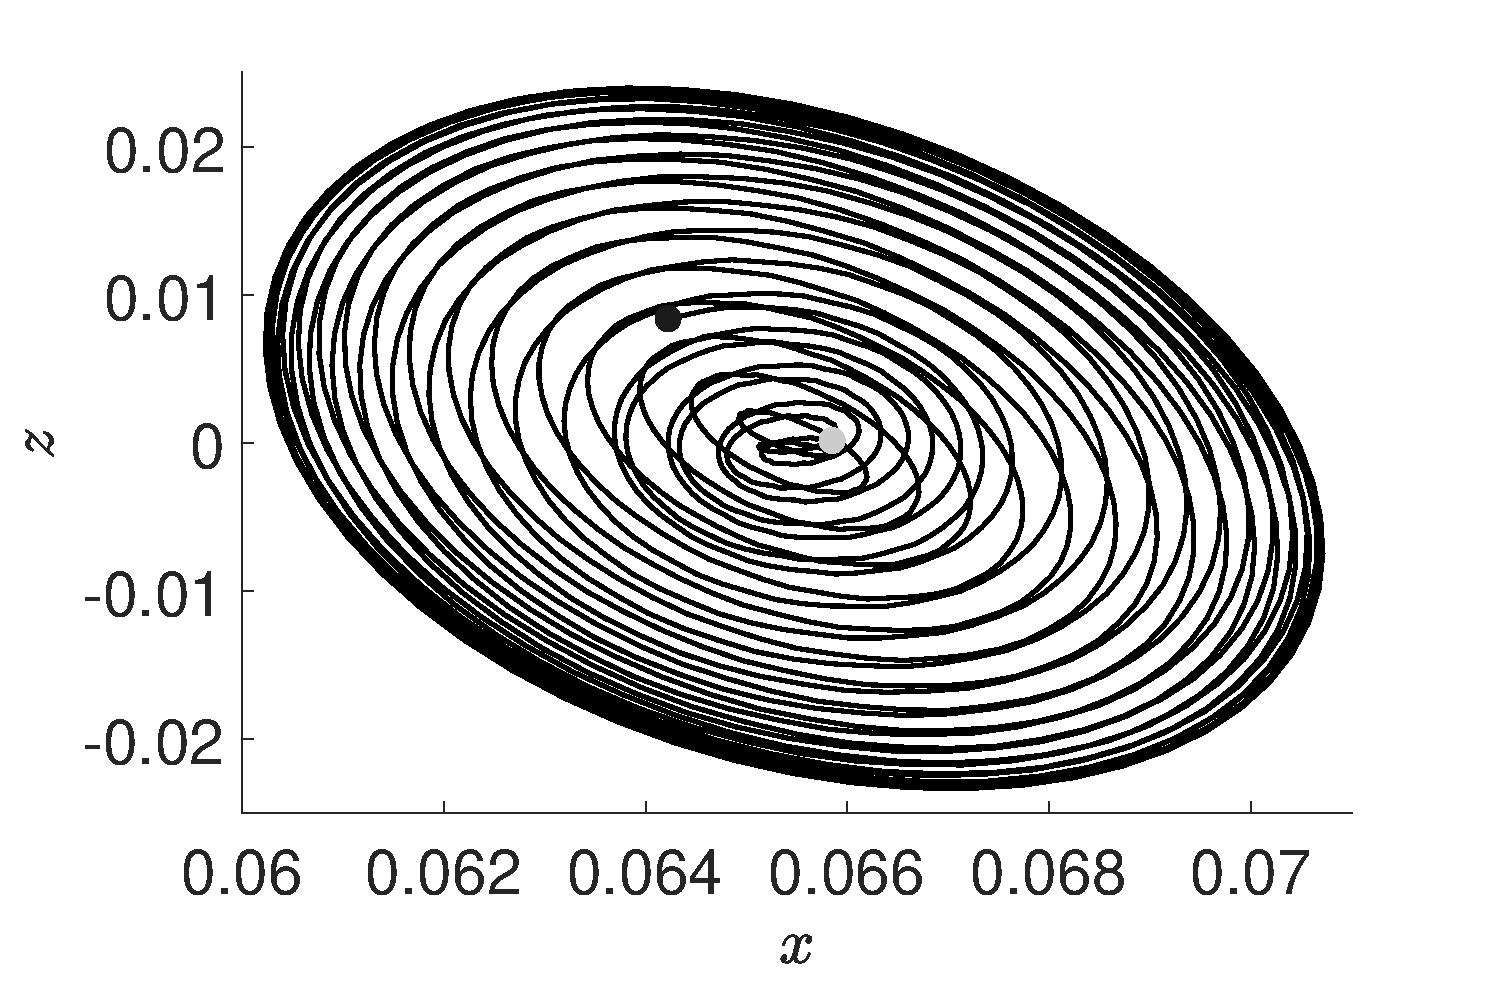
\includegraphics[width=.48\textwidth]{track_ep_pt1_tf_1_w_1pt703_kap_pt5_foc} & 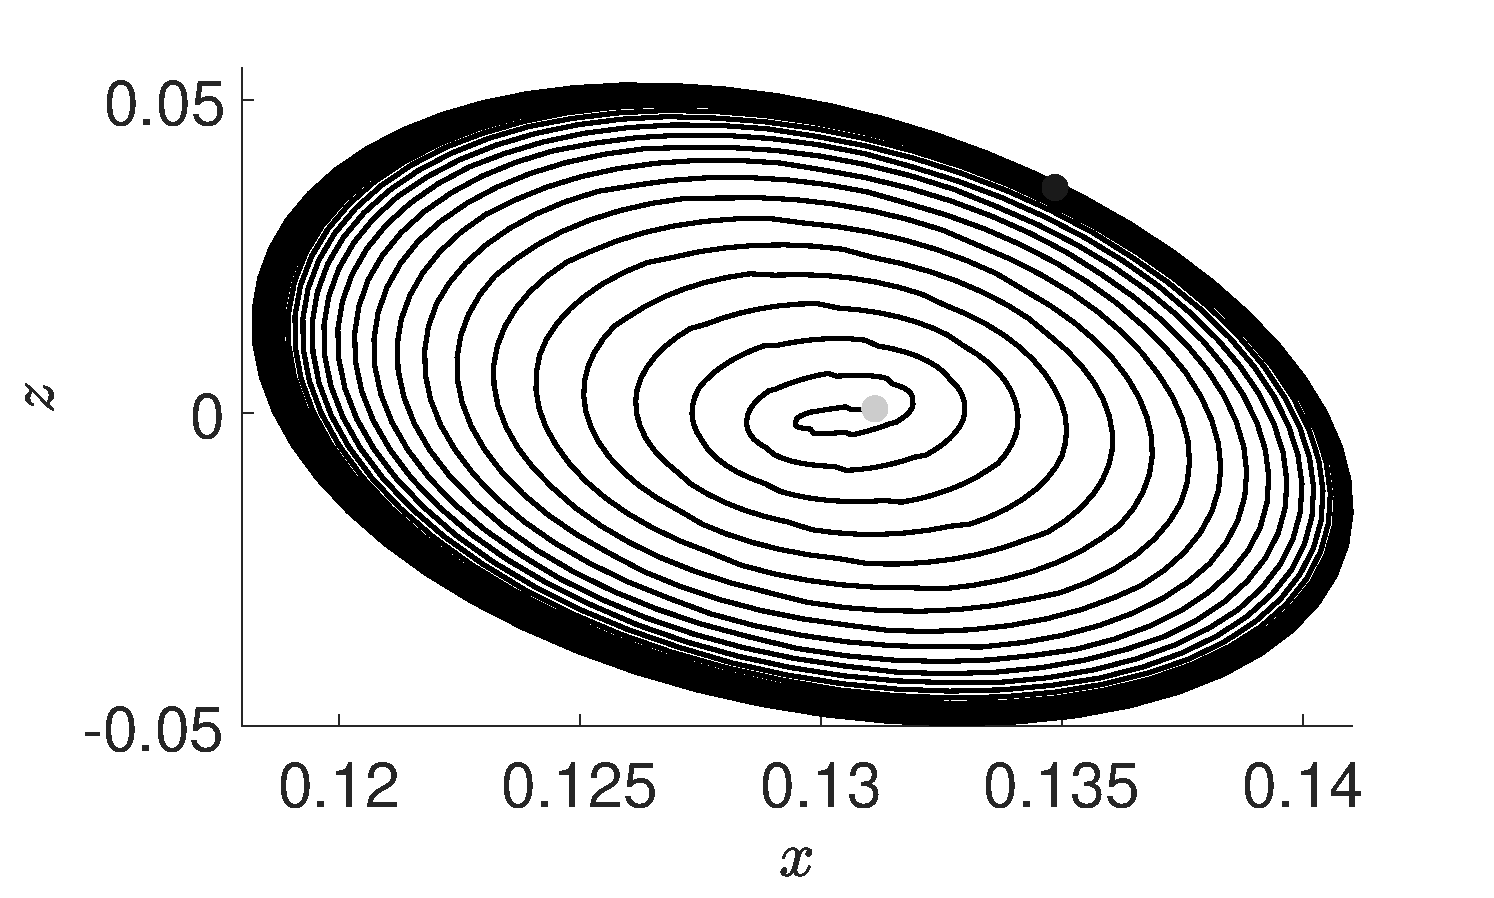
\includegraphics[width=.48\textwidth]{track_ep_pt1_tf_1_w_1pt667_kap_pt99_foc} \\
(a) $\omega=1.7027$ & (b) $\omega=1.6672$
\end{tabular}
\caption{\small {\bf Defocusing Case} - Plots of particle paths correspond to the solution given in Equation (\ref{snsolns}) with $\epsilon=0.1$, $\beta=1$, $k_{0}\approx 1$, with $\kappa=0.5$  (a), $\kappa=0.99$ (b). The choices of $\omega$ ensure that $\tilde{u}^{L}(1,\omega)=0$, see Figure \ref{fig:zerodriftk0}, thereby leading to the nearly closed, elliptical particle paths.  The grey dots indicate the starting positions of the tracers while the black dots indicate their final positions.  }
\label{fig:jaczerodrift}
\end{figure}
As can be seen, the particle paths, while not exactly closed, are spirals and are constrained in their horizontal and vertical extent by an outer elliptical perimeter.  Similarly, the shear strength can be chosen so that the LDV is zeroed out for the plane-wave solutions.  Taking $k_{0}=1$ and $A=1$, this corresponds to choosing $\omega = 1.6828$.  Figure \ref{fig:pwavezdrift} shows a nearly closed particle path.  We emphasize that these results are a confirmation of the predictions made in Figure \ref{fig:zerodriftk0}.  Thus, these numerical results validate our choice to generalize the GLM approach in so far as we see the generalization provides the correct predictions for when shear will quench surface drift.
\begin{figure}
\centering
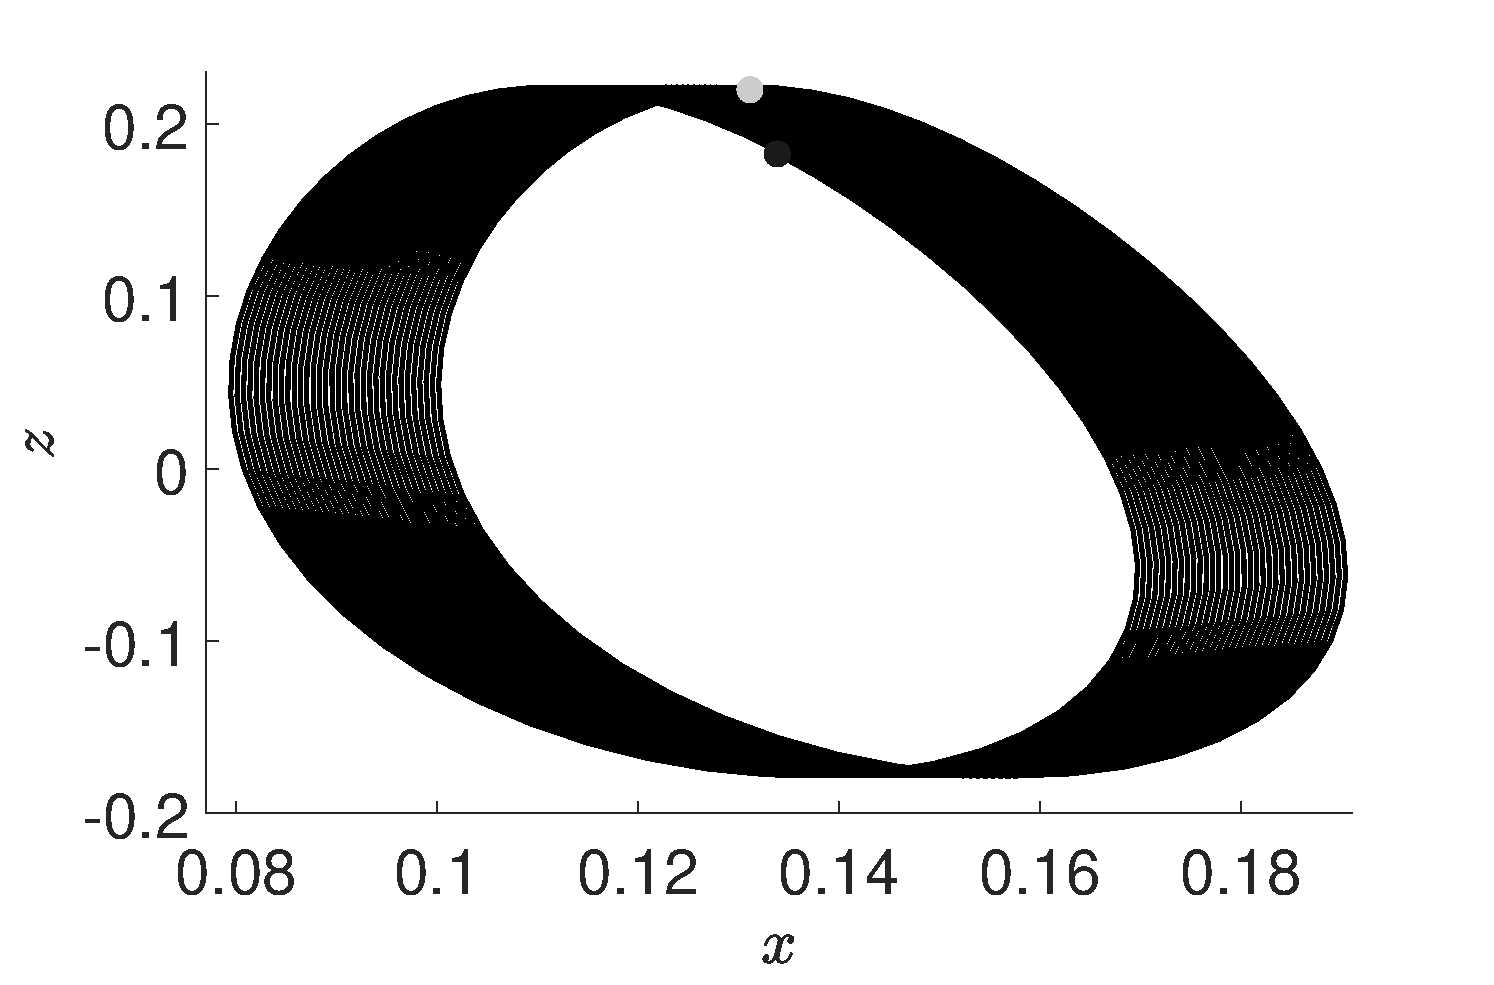
\includegraphics[width=.48\textwidth]{om_val_1pt7_k0_1_ep_pt1_defoc_ztrack_pwave}
\caption{\small {\bf Defocusing Case} - Plot of a particle path corresponding to a plane-wave solution with $\epsilon=0.1$, $A=1$, $k_{0}=1$ , and $\omega=1.6818$, which ensures that $\tilde{u}^{L}(1,\omega)=0$, see Figure \ref{fig:zerodriftk0}, thereby leading to the nearly closed, elliptical particle paths.  The grey dots indicate the starting positions of the tracers while the black dots indicate their final positions.  }
\label{fig:pwavezdrift}
\end{figure}

In some respects then, we have also shown that by appropriately choosing the shear, we can replicate the dynamics of a Gerstner wave, see \cite{constantin} by looking instead at a plane-wave solution moving over a counter-propagating shear current.  This could point towards resolving some of the questions raised in \cite{monismith,smith}, though this is a subject of future research.

Looking beyond cases in which Eulerian counterflows quench drift, we now consider the defocusing NLS Jacobi elliptic function solutions given in Equation \eqref{snsolns}.  We choose $k_{0}\approx1$, $\epsilon=0.1$, $\kappa=0.99$ (near the dark-soliton limit).  Solving the dynamical system for the particle paths up to time $t=1/\epsilon^{2}$ generates Figure \ref{fig:defoc_kap_pt99} (a) and (b) for $\omega= 1.17$ and $\omega= 4$ respectively.  While the particle path motion seen in Figure \ref{fig:defoc_kap_pt99}(a) is rapidly oscillating, the net transport and amplitude is quite small.
\begin{figure}
\centering
\begin{tabular}{cc}
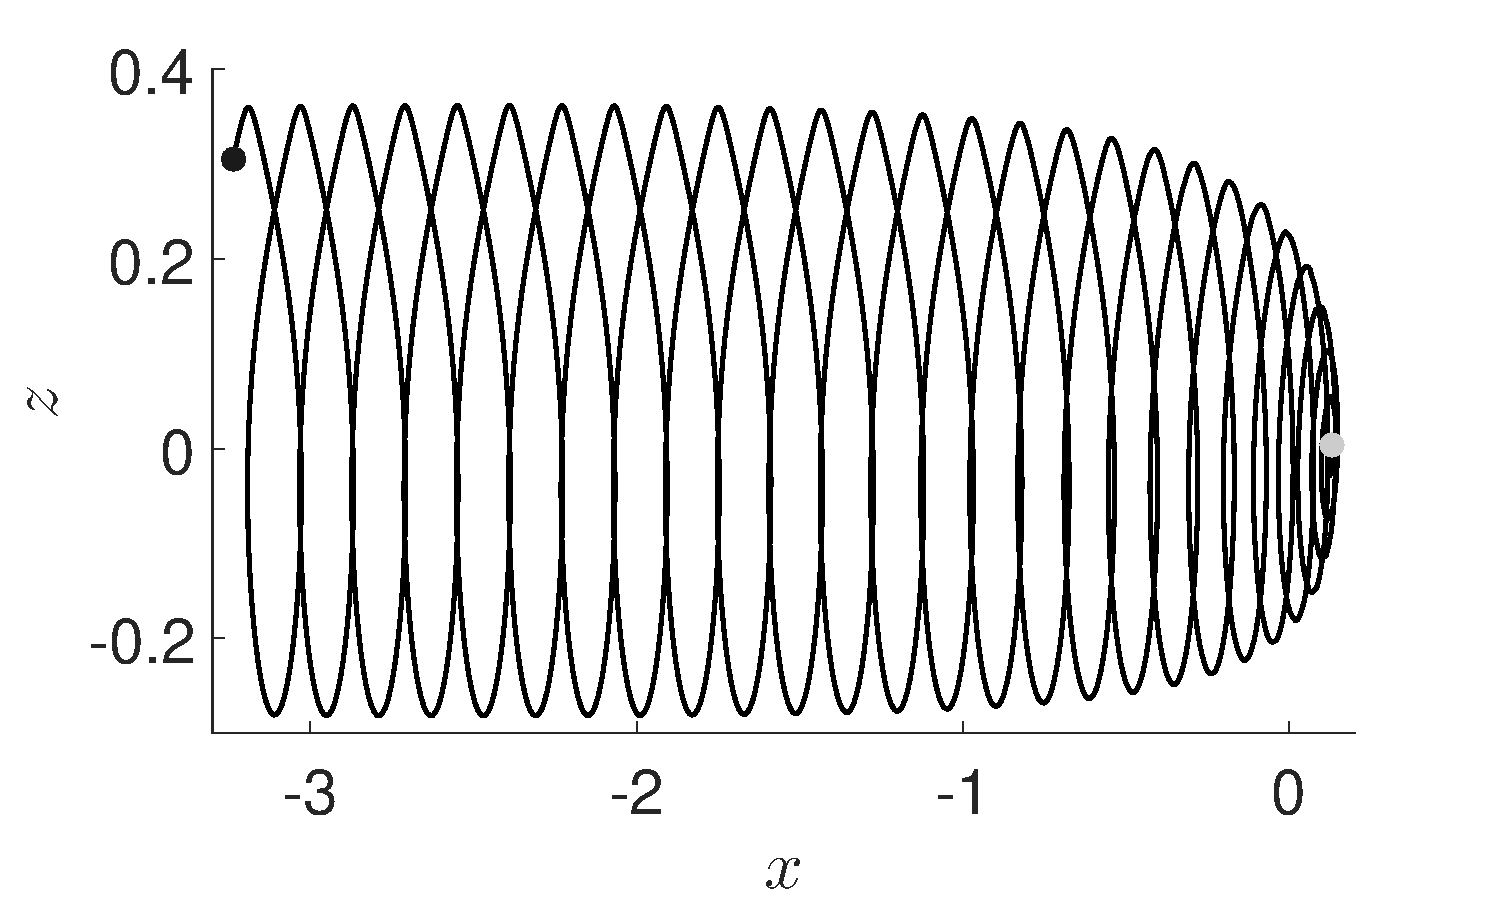
\includegraphics[width=.48\textwidth]{om_val_1pt17_k0_1_ep_pt1_defoc_ztrack} &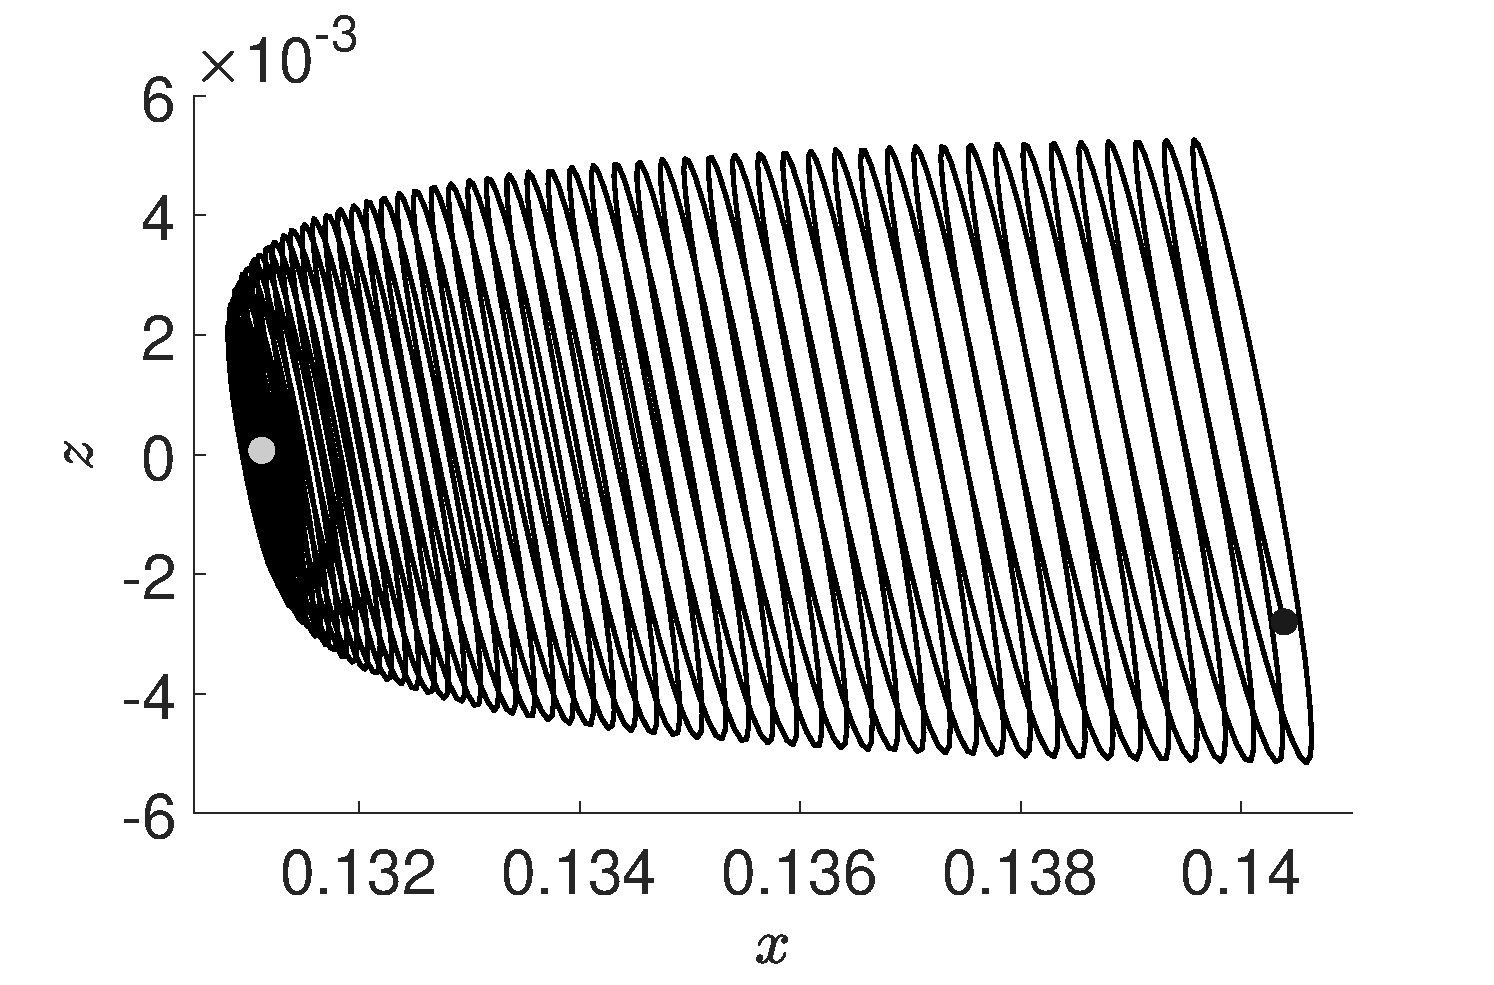
\includegraphics[width=.48\textwidth]{om_val_4_k0_1_ep_pt1_defoc_ztrack} \\
(a) $\omega = 1.17$ & (b) $\omega=4$
\end{tabular}
\caption{\small {\bf Defocusing} - Near dark soliton solution for $k_{0}\approx1$, $\kappa=.99$ and $\omega=1.17$ (a) and $\omega=4$ (b).  The grey dot indicates the starting position of the tracer while the black dot indicates the final position.}
\label{fig:defoc_kap_pt99}
\end{figure}

However, if $\omega=4$ in the case of a plane wave, we do not necessarily get the same diminished response seen for the Jacobi elliptic solutions; see Figure \ref{fig:defoc_pwave}.  The highly oscillatory plane-wave profile induces a particle path which ultimately exhibits a strong rightward drift which follows the strong counter-propagating shear current.   The associated SDV and LDV at the surface for the plane wave with these parameters are given by
\begin{align*}
\bar{u}^{S}_{s} = & -8.4985\epsilon^{2} + \mathcal{O}(\epsilon^{3}),\\
\bar{u}^{L}_{s} = & 29.2719\epsilon^{2} + \mathcal{O}(\epsilon^{3}).
\end{align*}
This explains the stronger net rightward drift of the particle shown in Figure \ref{fig:defoc_pwave}.  Finally, note that this shows the SDV and the LDV can oppose one another, thereby clarifying the need to use both velocities to fully understand the drift properties associated with a surface wave.
 \begin{figure}
\centering
\begin{tabular}{cc}
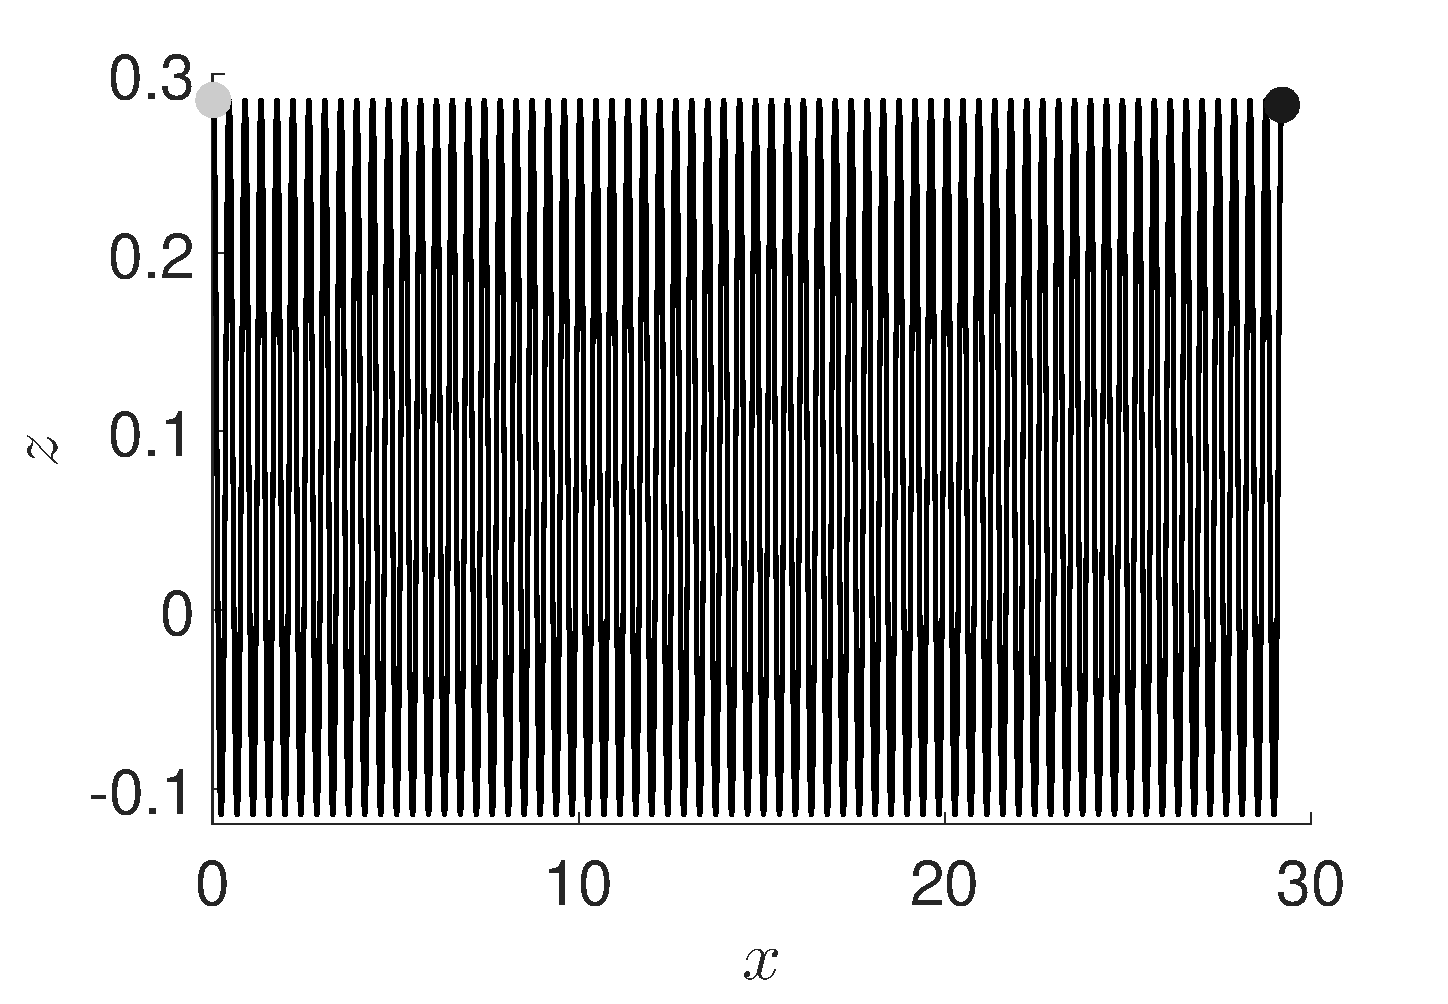
\includegraphics[width=.5\textwidth]{om_val_4_k0_1_ep_pt1_defoc_ztrack_pwave} & 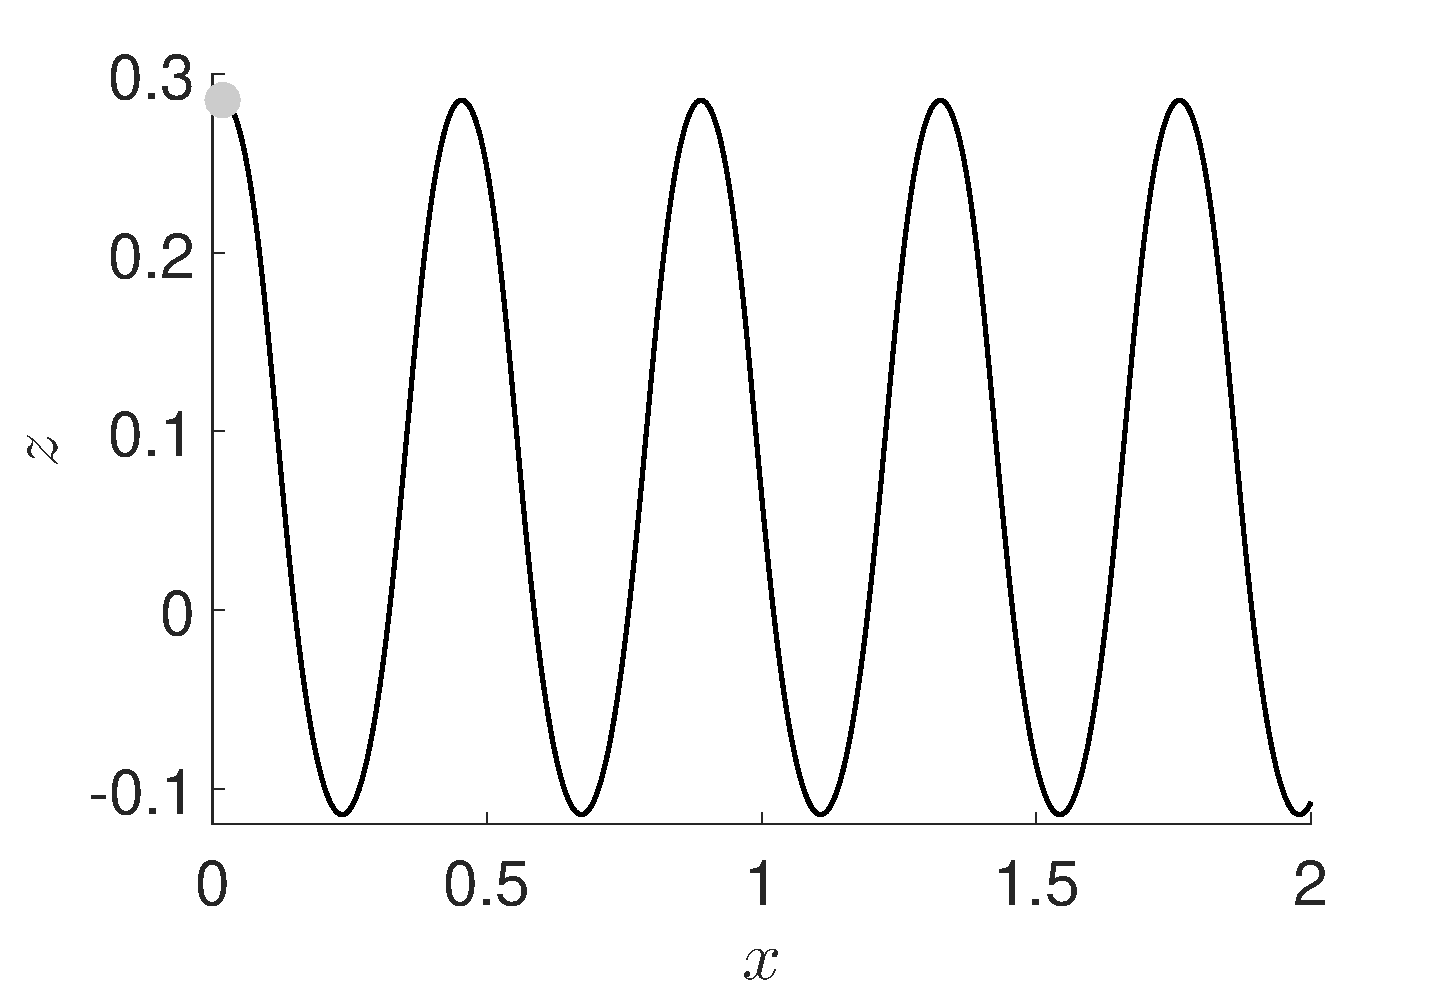
\includegraphics[width=.5\textwidth]{om_val_4_k0_1_ep_pt1_defoc_ztrack_pwave_detail}\\
(a) & (b)
\end{tabular}
\caption{\small {\bf Defocusing Case} - Plane-wave solution for $k_{0}=1$, $\omega=4$, $A=1$, with (b) providing a detail of (a).  The grey dot indicates the starting position of the tracer while the black dot indicates the final position.}
\label{fig:defoc_pwave}
\end{figure}

\section{Conclusion and Future Directions}

In this paper, to better understand the transport properties of nonlinear waves moving over constant-vorticity currents, we have derived an asymptotically self-consistent higher-order model for the interaction between the mean wave height and the leading order modulated carrier wave in the presence of surface tension and a constant vorticity current.  Using this, a NLS equation is derived, and the role of surface tension in determining the existence of modulational instability is fully explored.  A formula for the Stokes drift velocity at the surface is derived allowing for the identification of shear profiles which enhance or quench horizontal surface transport.  Numerical simulations corroborate the surface theory developed in this paper.

The work in this paper provides possible explanatory mechanisms for otherwise unexplained oceanic phenomena observed 
in \cite{smith} and justification for phenomenological choices in oceanographic modeling put forward in \cite{breivik}.  Assessing how accurate a constant-vorticity-modulational-nonlinear wave model describes these real world problems is an important future research direction.  Likewise, while a higher-order model describing the coupled evolution of the mean and modulated carrier wave is derived, the properties of this equation are not studied directly.  

\section{Acknowledgments}
This material is based upon work supported by the National Science Foundation under Grant No. DMS-1439786 while CWC and JDC were in residence at the Institute for Computational and Experimental Research in Mathematics in Providence, RI, during the Spring 2017 semester.  Additionally, JDC acknowledges and thanks the Norwegian Fulbright Core Scholar Program for supporting his five-month long visit to the University of Bergen to work with HK. This research was also supported by
the Research Council of Norway through grants 213474/F20 and 239033/F20.

\bibliographystyle{JFM_Style/jfm}
\bibliography{deep_water_shear_Feb2}
\end{document}
